\documentclass{ieeeaccess}
\usepackage[utf8]{inputenc}
\usepackage{cite}
\usepackage{amsmath,amssymb,amsfonts}
\usepackage{graphicx}
\usepackage{textcomp}
\usepackage{booktabs}
\usepackage{microtype}
\usepackage{ragged2e}
\usepackage{tikz}
\usetikzlibrary{arrows.meta, positioning, fit, backgrounds, calc}
\usepackage[english]{babel}
\addto\captionsenglish{\renewcommand{\refname}{References}}

% [FIX] tikz loads xcolor, which breaks the class's PANTONE spot color
% "accessblue" (Incompatible color definition). Without it, the TITLE and the
% blue ABSTRACT / INDEX TERMS labels become invisible. We redefine accessblue
% with the same CMYK as the PANTONE 3015 C used by the class (AddSpotColor line).
\definecolor{accessblue}{cmyk}{1,0.3,0,0.2}

% Grayscale palette + highlight for the block diagrams
\definecolor{blkBase}{RGB}{237,237,237}   % light gray (common blocks)
\definecolor{blkEdge}{RGB}{120,120,120}   % gray border
\definecolor{blkHi}{RGB}{196,210,225}     % highlight (desaturated slate blue)
\definecolor{blkHiEdge}{RGB}{82,110,143}  % highlight border

\usepackage{bm}
\makeatletter
\AtBeginDocument{\DeclareMathVersion{bold}
\SetSymbolFont{operators}{bold}{T1}{times}{b}{n}
\SetSymbolFont{NewLetters}{bold}{T1}{times}{b}{it}
\SetMathAlphabet{\mathrm}{bold}{T1}{times}{b}{n}
\SetMathAlphabet{\mathit}{bold}{T1}{times}{b}{it}
\SetMathAlphabet{\mathbf}{bold}{T1}{times}{b}{n}
\SetMathAlphabet{\mathtt}{bold}{OT1}{pcr}{b}{n}
\SetSymbolFont{symbols}{bold}{OMS}{cmsy}{b}{n}
\renewcommand\boldmath{\@nomath\boldmath\mathversion{bold}}}
\makeatother

\graphicspath{{images/}}

\setlength{\emergencystretch}{3em}

\def\BibTeX{{\rm B\kern-.05em{\sc i\kern-.025em b}\kern-.08em
    T\kern-.1667em\lower.7ex\hbox{E}\kern-.125emX}}

\begin{document}
\history{}
\doi{}

\title{System Identification and Modeling of a Hybrid VTOL Unmanned Aerial Vehicle (UAV) in Quadrotor Mode}

\author{\uppercase{Henrique Mark dos Santos Corrêa}\authorrefmark{1} and
\uppercase{Neusa Maria Franco de Oliveira}\authorrefmark{1}}

\address[1]{Department of Electronic Engineering (IEE), Instituto Tecnológico de Aeronáutica (ITA), São José dos Campos, SP 12228-900, Brazil (e-mail: henriquecorrea@ita.br; neusa@ita.br)}

\tfootnote{Work developed within the graduate program in Electronic and Computer Engineering of the Instituto Tecnológico de Aeronáutica (ITA).}

\markboth
{Corrêa \MakeLowercase{\textit{et al.}}: System Identification and Modeling of a Hybrid VTOL UAV in Quadrotor Mode}
{Corrêa \MakeLowercase{\textit{et al.}}: System Identification and Modeling of a Hybrid VTOL UAV in Quadrotor Mode}

\corresp{Corresponding author: Henrique Mark dos Santos Corrêa (e-mail: henriquecorrea@ita.br).}

\begin{abstract}
This work describes the system identification and validation of a nonlinear mathematical model for the quadrotor flight mode of a hybrid-configuration VTOL Unmanned Aerial Vehicle (UAV). The main objective is to obtain an identified model of the quadrotor mode that serves as a basis for developing control algorithms and an autopilot (AP) for the vertical takeoff and landing phases. The M4V (Maneuver, Measurements, Methods, Models) system identification methodology was applied, using data collected in real flights. To estimate the inertia parameters and the aerodynamic coefficients, a time-domain nonlinear least-squares optimization method was employed, which minimizes the error between the simulated response and the data measured during maneuvers that excited the aircraft modes. The identified model was validated by comparing its responses with a distinct set of flight data not used in the estimation. The results demonstrate good correlation between the real and simulated data, confirming the adequacy of the model for the intended control applications.
\end{abstract}

\begin{keywords}
System identification, output-error method (OEM), dynamic modeling, quadrotor mode, hybrid VTOL UAV.
\end{keywords}

\titlepgskip=-21pt

\maketitle

\section{Introduction}
\label{sec:introducao}

\PARstart{U}{nmanned} aerial vehicles (UAVs) with vertical takeoff and landing (VTOL) capability have gained prominence due to their versatility, combining the cruise efficiency of a fixed-wing aircraft with the operational flexibility of a multirotor~\cite{c1}. The aircraft that is the subject of this study, the DH Hybrid-Drone VTOL, is a hybrid-configuration UAV capable of transitioning between quadrotor flight mode and fixed-wing mode. Figure~\ref{fig:fases_voo} illustrates the typical flight phases of this type of aircraft, from vertical takeoff to landing, passing through the transition and the fixed-wing cruise.

Although the aircraft operates in multiple flight modes, the vertical takeoff and landing phases are performed exclusively in quadrotor mode and constitute an important stage for autonomous operation. In this context, the present work focuses on the identification of the dynamic model of the quadrotor mode, taking into account the particularities of a hybrid VTOL platform, such as the asymmetric mass distribution arising from the H-frame configuration and its influence on the aircraft's moments of inertia.

\begin{figure}[!htbp]
      \centering
      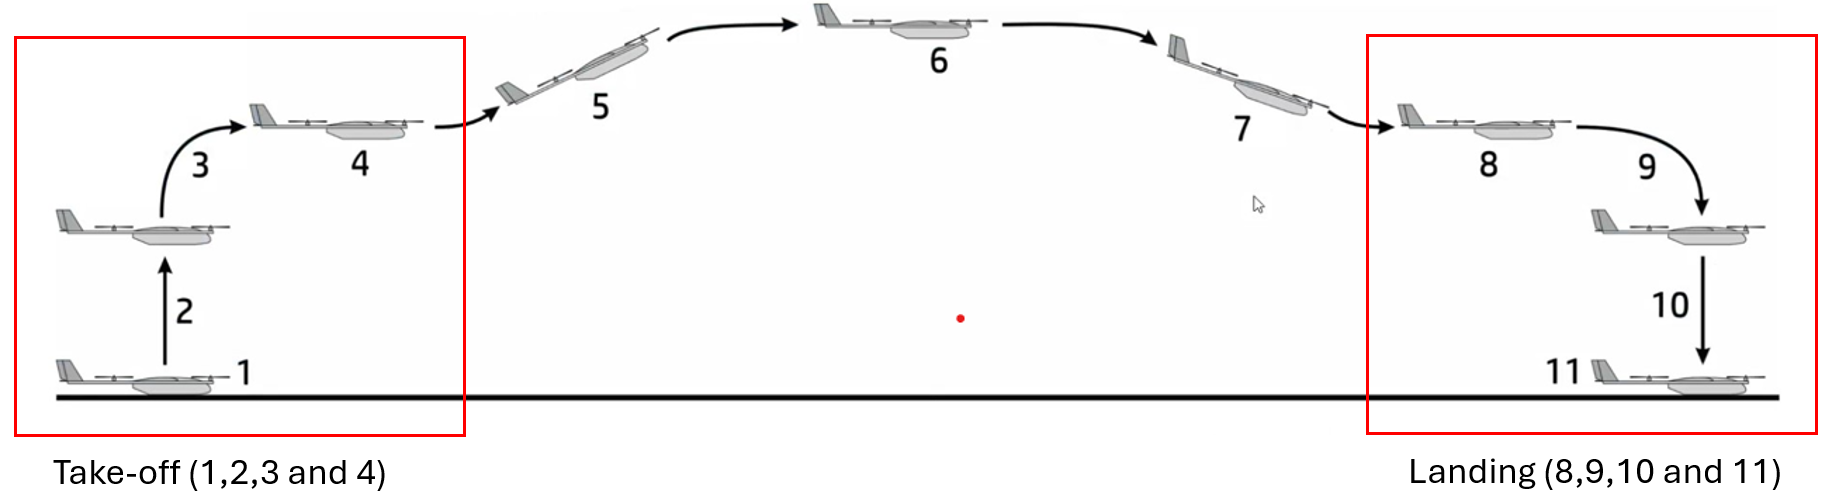
\includegraphics[width=\columnwidth]{passos.png}
      \caption{Illustration of the flight phases of a hybrid VTOL.}
      \label{fig:fases_voo}
\end{figure}

The main objective is to obtain, from real flight data, an identified nonlinear mathematical model that faithfully represents the dynamics of the quadrotor mode. This model will serve as a basis for developing control algorithms and an autopilot (AP) for the autonomous vertical takeoff and landing maneuvers. The identification is carried out from initial values obtained from the characterization of the motors, with the thrust and reaction-torque curves of the motors obtained on a bench, from the aircraft's moments of inertia obtained in simulation software, and from data collected in specific flight maneuvers.

\section{M4V Identification Method}
\label{sec:m4v}

For the system identification, the M4V (Maneuver, Measurements, Methods, Models, Validation) methodology was used, a structured approach widely employed in the identification of aerial vehicle systems~\cite{c2}. The M4V methodology divides the identification process into well-defined phases, ensuring a systematic and robust approach.

\begin{figure}[!htbp]
      \centering
      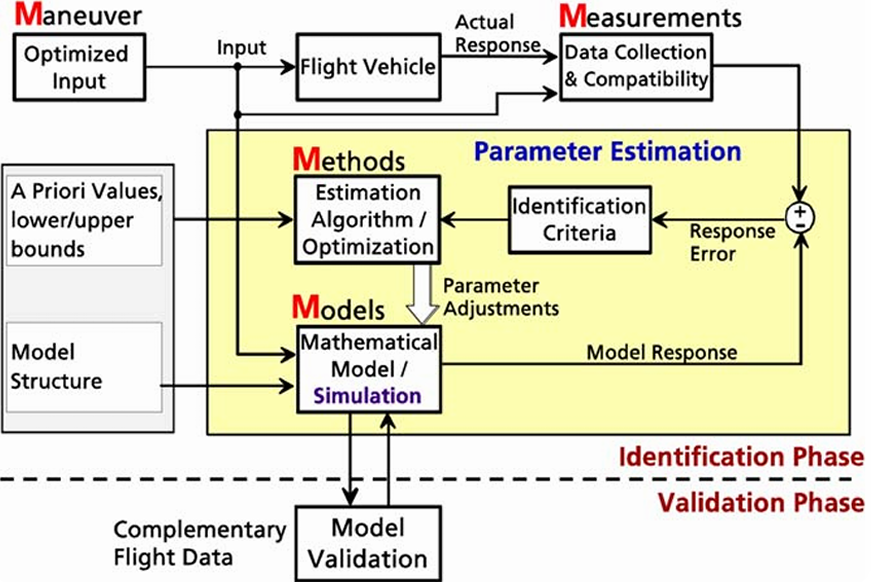
\includegraphics[width=\columnwidth]{m4m.png}
      \caption{Diagram of the M4V method.}
      \label{fig:m4v}
\end{figure}

\begin{RaggedRight}
The phases of the M4V methodology are:
\begin{itemize}
    \item \textbf{Maneuver:} Optimized inputs are designed and applied to the vehicle in flight to adequately excite its dynamics.
    \item \textbf{Measurements:} The data of the aircraft's actual response to the maneuvers are collected through onboard sensors. Data compatibility and quality are verified in this phase.
    \item \textbf{Methods:} Estimation and optimization algorithms are used to identify the parameters of the mathematical model. The fit is performed based on identification criteria, in particular the minimization of the error between the actual and simulated responses.
    \item \textbf{Models:} A structural mathematical model, with initial (a priori) values, is continuously refined with the estimated parameters until the error is minimized.
\end{itemize}
\end{RaggedRight}

After the identification phase, the obtained model is subjected to a validation phase, in which complementary flight data, not used in the estimation, are used to verify the predictive capability and robustness of the model.

\section{Mathematical Model of the Quadrotor Mode}
\label{sec:modelo}

The mathematical model was developed considering the aircraft as a 6-DOF rigid body operating in quadrotor mode. In this mode, lift and attitude control are performed exclusively by the four vertical motors, while the rear cruise motor and the aerodynamic surfaces remain inactive. Although the hybrid VTOL configuration introduces particularities in the mass distribution and geometry of the aircraft relative to a conventional quadrotor, the dynamics in this mode are governed solely by the forces and moments generated by the vertical rotors. Figures~\ref{fig:drone_config} and~\ref{fig:drone_real} illustrate the layout of the motors, with the moments and forces they apply to the aircraft.

\begin{figure}[!htbp]
      \centering
      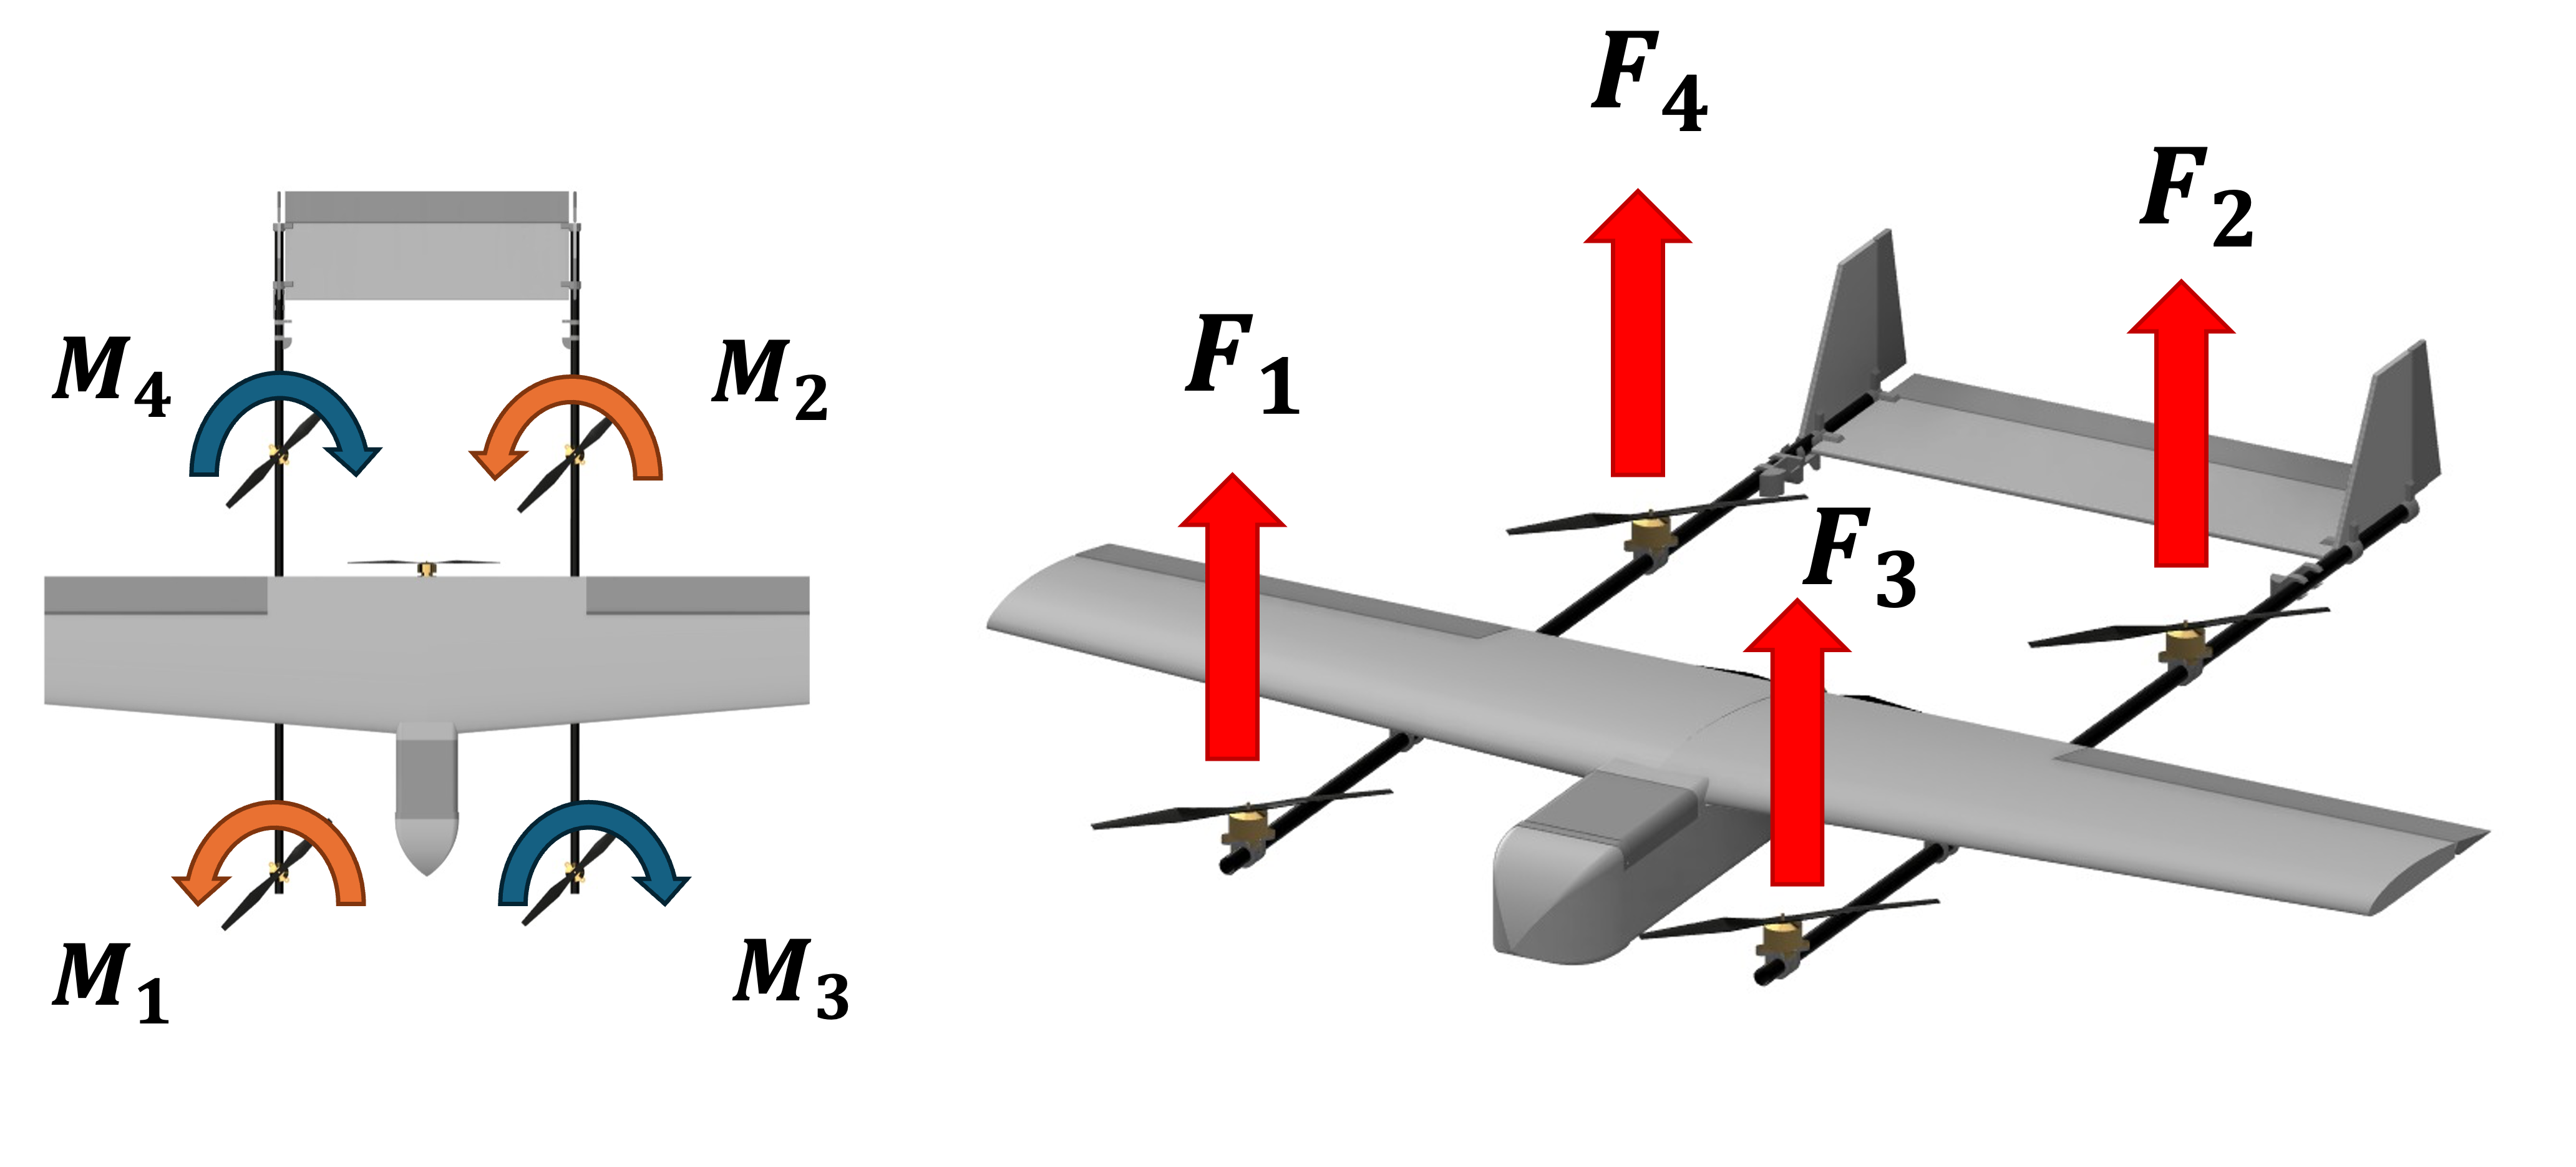
\includegraphics[width=\columnwidth]{forcas-momentos.png}
      \caption{Relationship of moments and forces applied by the motors.}
      \label{fig:drone_config}
\end{figure}

\begin{figure}[!htbp]
      \centering
      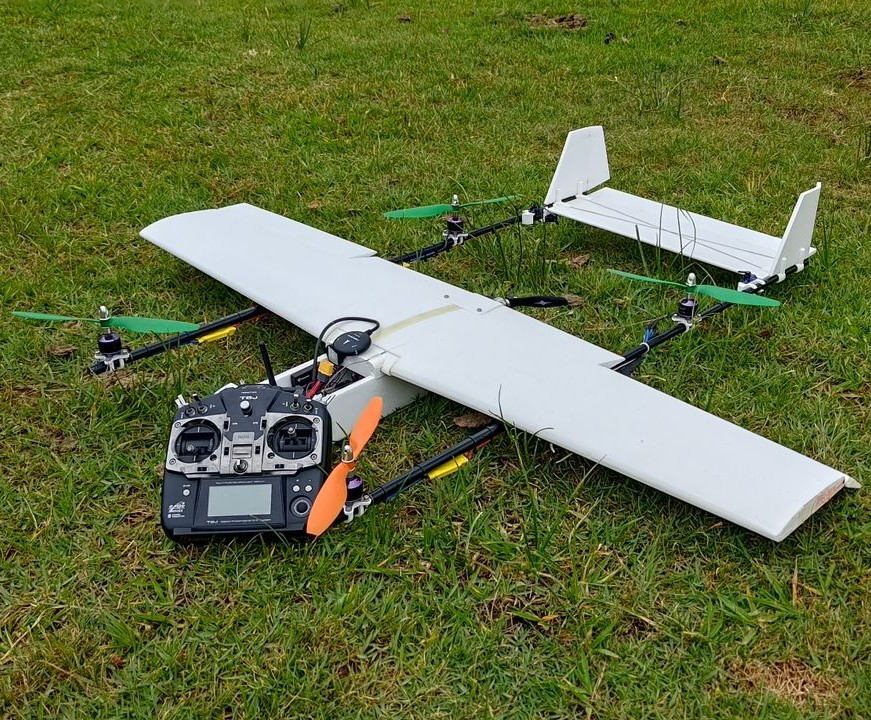
\includegraphics[width=\columnwidth]{rdrone.jpeg}
      \caption{DH Hybrid-Drone VTOL aircraft.}
      \label{fig:drone_real}
\end{figure}

The model is described by a set of nonlinear state equations. The state vector $\mathbf{x}$ and input vector $\mathbf{u}$ are defined as:
\begin{equation}
    \mathbf{x} = [\phi, \theta, \psi, p, q, r, u, v, w]^T
\end{equation}
\begin{equation}
    \mathbf{u} = [\sigma_1, \sigma_2, \sigma_3, \sigma_4]^T
\end{equation}
where $\phi, \theta, \psi$ are the Euler angles (roll, pitch, and yaw); $p, q, r$ are the angular rates in the body frame; $u, v, w$ are the linear velocities in the body-axis system; and $\sigma_i$ are the normalized PWM commands sent to the four motors of the multirotor~\cite{c3}, detailed below in the motor model.

This complete mathematical model is divided into three parts: first the motor model and the aggregate generation of the instantaneous forces and moments, then the rigid-body dynamics, which are separated into a rotational model and a translational model. Figure~\ref{fig:model_diagram} summarizes this structure in blocks, from the motor command to the outputs of the rigid-body dynamics.

\begin{figure}[!t]
\centering
\resizebox{\columnwidth}{!}{%
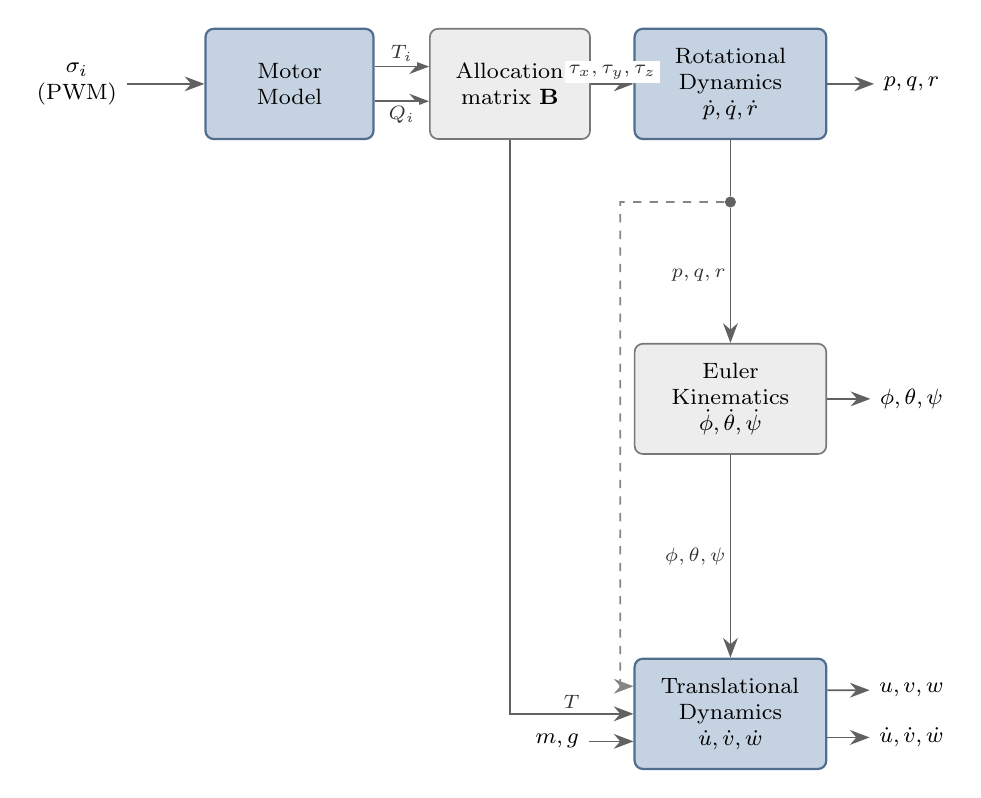
\begin{tikzpicture}[
    sysblock/.style={rectangle, draw=blkEdge, semithick, fill=blkBase, rounded corners=3pt, minimum height=1.4cm, text width=2.2cm, align=center, font=\footnotesize},
    hi/.style={fill=blkHi, draw=blkHiEdge, thick},
    io/.style={font=\footnotesize},
    arr/.style={-{Stealth[length=2.5mm]}, semithick, black!62},
    darr/.style={-{Stealth[length=2.5mm]}, semithick, black!48, dashed},
    lbl/.style={font=\scriptsize, fill=white, inner sep=1.5pt, text=black!80},
    dot/.style={circle, fill=black!62, inner sep=0pt, minimum size=4pt},
]

% ========== ROW 1 (y=0): sigma (PWM) -> Motor Model -> (T_i,Q_i) -> B -> RotDyn ==========
\node[io, align=center] at (0,0) (sig) {$\sigma_i$\\(PWM)};
\node[sysblock, hi, text width=1.9cm] at (2.7,0) (motor) {Motor\\Model};
\node[sysblock, text width=1.8cm] at (5.5,0) (balloc) {Allocation\\matrix $\mathbf{B}$};
\node[sysblock, hi] at (8.3,0) (rotdyn) {Rotational\\Dynamics\\$\dot{p},\dot{q},\dot{r}$};

\draw[arr] (sig) -- (motor);
\draw[arr] ([yshift=0.22cm]motor.east) -- node[lbl, above] {$T_i$} ([yshift=0.22cm]balloc.west);
\draw[arr] ([yshift=-0.22cm]motor.east) -- node[lbl, below] {$Q_i$} ([yshift=-0.22cm]balloc.west);
\draw[arr] (balloc) -- node[lbl, above] {$\tau_x,\tau_y,\tau_z$} (rotdyn);

% Output p,q,r
\node[io] at (10.6,0) (pqr_out) {$p, q, r$};
\draw[arr] (rotdyn) -- (pqr_out);

% ========== ROW 2 (y=-4): Euler ==========
\node[sysblock] at (8.3,-4) (euler) {Euler\\Kinematics\\$\dot{\phi},\dot{\theta},\dot{\psi}$};
\node[io] at (10.6,-4) (att_out) {$\phi, \theta, \psi$};
\draw[arr] (euler) -- (att_out);

% ========== ROW 3 (y=-8): TransDyn ==========
\node[sysblock, hi] at (8.3,-8) (transdyn) {Translational\\Dynamics\\$\dot{u},\dot{v},\dot{w}$};
\node[io] at (10.6,-7.7) (uvw_out) {$u, v, w$};
\node[io] at (10.6,-8.3) (acc_out) {$\dot{u}, \dot{v}, \dot{w}$};
\draw[arr] ([yshift=0.3cm]transdyn.east) -- (uvw_out);
\draw[arr] ([yshift=-0.3cm]transdyn.east) -- (acc_out);

% m, g input (enters bottom of west side)
\node[io] at (6.1,-8.35) (const) {$m, g$};
\draw[arr] (const) -- ([yshift=-0.35cm]transdyn.west);

% ========== CONNECTIONS ==========

% --- Empuxo total T: B -> TransDyn (solid, down, enters west middle) ---
\draw[arr] (balloc.south) -- (5.5,-8.0) -- node[lbl, above] {$T$} ([yshift=0.0cm]transdyn.west);

% --- RotDyn -> Euler (solid, center vertical) ---
\node[dot] at (8.3,-1.5) (junc) {};
\draw[semithick, black!62] (rotdyn.south) -- (junc);
\draw[arr] (junc) -- node[lbl, left] {$p,q,r$} (euler.north);

% --- p,q,r -> TransDyn (dashed, enters west top) ---
\draw[darr] (junc.west) -- (6.9,-1.5) -- (6.9,-7.65) -- ([yshift=0.35cm]transdyn.west);

% --- Euler -> TransDyn (solid, center) ---
\draw[arr] (euler.south) -- node[lbl, left] {$\phi,\theta,\psi$} (transdyn.north);

\end{tikzpicture}%
}
\caption{Block diagram of the DH dynamic model with the three subsystems: Motor Model, Rotational Model, and Translational Model.}
\label{fig:model_diagram}
\end{figure}

\subsection{Motor Model}

The motor model describes the chain that converts the PWM command applied to each motor into the generalized efforts applied to the rigid body. First, the normalized PWM command $\sigma_i$ is converted into the rotor angular rate $\Omega_i$, which produces the thrust $T_i$ and the reaction torque $Q_i$; these individual efforts are then finally combined by the allocation matrix $\mathbf{B}$ into the total thrust $T$ and the moments $\tau_x$, $\tau_y$, and $\tau_z$~\cite{c13}. Figure~\ref{fig:blocos_motor} presents the two-stage structure of this model, including the first-order dynamics that models the delay in the motor response.

Both the input and output values were obtained from tests on a dynamometer bench, which related the input command to the rotor angular rate, thrust, and reaction torque generated with the propeller attached, all with the battery fully charged in order to disregard the effects of power loss, simplifying the analysis.

\begin{figure}[!htbp]
      \centering
      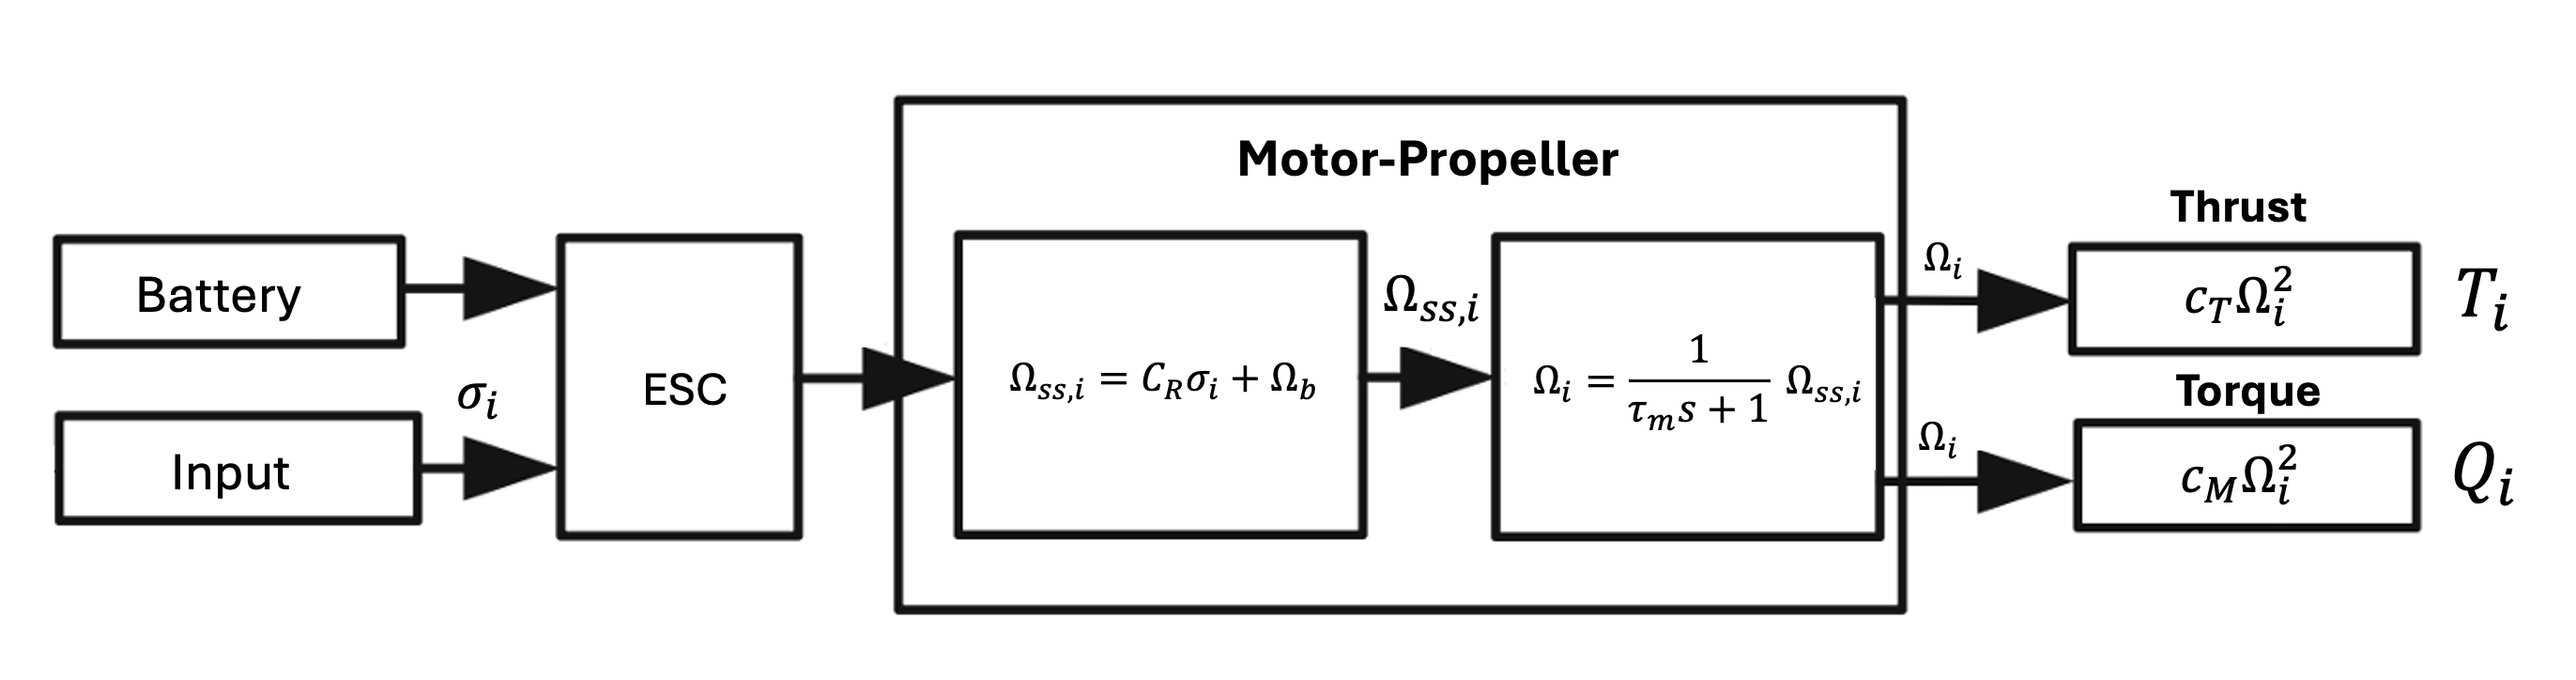
\includegraphics[width=\columnwidth]{blocos-motor.png}
      \caption{Block diagram of the motor model: the ESC converts the normalized command $\sigma_i$ into the steady-state angular rate (Equation~\eqref{eq:omega-ss}), filtered by the first-order dynamics (Equation~\eqref{eq:omega-lag}) and transformed into thrust and reaction torque (Equation~\eqref{eq:tq}). Adapted from~\cite{c13}.}
      \label{fig:blocos_motor}
\end{figure}

The command of each motor is the pulse width $\delta_{PWM,i}$, normalized to the interval $[0,1]$:
\begin{equation}
\sigma_i = \frac{\delta_{PWM,i} - \delta_{\min}}{\delta_{\max} - \delta_{\min}}
\label{eq:norm}
\end{equation}
where $\delta_{\min} = 1000~\mu$s and $\delta_{\max} = 2000~\mu$s are the limits of the ESC operating range.

The first stage of the chain relates the normalized command to the rotor angular rate. In steady state, the bench data of Figure~\ref{fig:motor_pwm_rpm} show that this relationship is well approximated by a straight line~\cite{c13}:
\begin{equation}
\Omega_{ss,i} = C_R\,\sigma_i + \Omega_b
\label{eq:omega-ss}
\end{equation}
where $C_R$ is the gain of the ESC--motor assembly and $\Omega_b$ is the minimum operating angular rate. The least-squares fit to the measured points, excluding the motor-stopped point, results in $C_R = 4523$~RPM and $\Omega_b = 1837$~RPM.

\begin{figure}[!htbp]
      \centering
      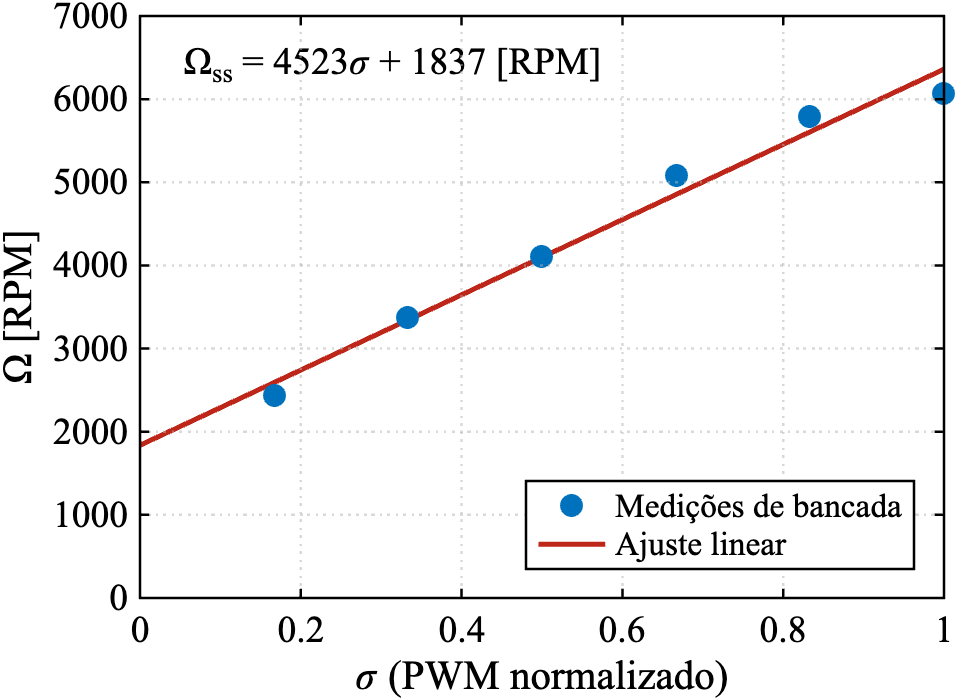
\includegraphics[width=\columnwidth]{motor_pwm_rpm.png}
      \caption{Steady-state rotor angular rate as a function of the normalized PWM command. The points are the bench measurements and the solid line is the linear fit of Equation~\eqref{eq:omega-ss}.}
      \label{fig:motor_pwm_rpm}
\end{figure}

However, the response of the ESC--motor--propeller assembly is not instantaneous: the angular rate converges to the steady-state value with a dynamics well approximated by a first-order system that, in the frequency domain, corresponds to a low-pass filter~\cite{c13}:
\begin{equation}
\Omega_i(s) = \frac{1}{\tau_m s + 1}\,\Omega_{ss,i}(s)
\label{eq:omega-lag}
\end{equation}
where $s$ is the Laplace variable and $\tau_m = 0.05$~s is the adopted time constant. The instantaneous angular rate $\Omega_i$ resulting from this dynamics is the quantity that effectively generates the rotor efforts.

Each rotor, spinning at rate $\Omega_i$, produces a thrust and a reaction torque proportional to the square of this rate~\cite{c11},~\cite{c13}:
\begin{equation}
T_i = c_{T_i}\,\Omega_i^{2}, \qquad Q_i = c_{M_i}\,\Omega_i^{2}
\label{eq:tq}
\end{equation}
where $c_{T_i}$ and $c_{M_i}$ are the thrust and torque coefficients, which depend on the propeller geometry and the air density, treated as identifiable parameters of the model. The quadratic fit to the bench data, presented in Figure~\ref{fig:motor_tq}, provides the reference values $c_T = 1.76\times10^{-7}$~N/RPM$^2$ and $c_M = 5.04\times10^{-9}$~N$\cdot$m/RPM$^2$, adopted as initial values of the identification process (Table~\ref{tab:const_iniciais}), in which they are refined individually for each motor.

\begin{figure}[!htbp]
      \centering
      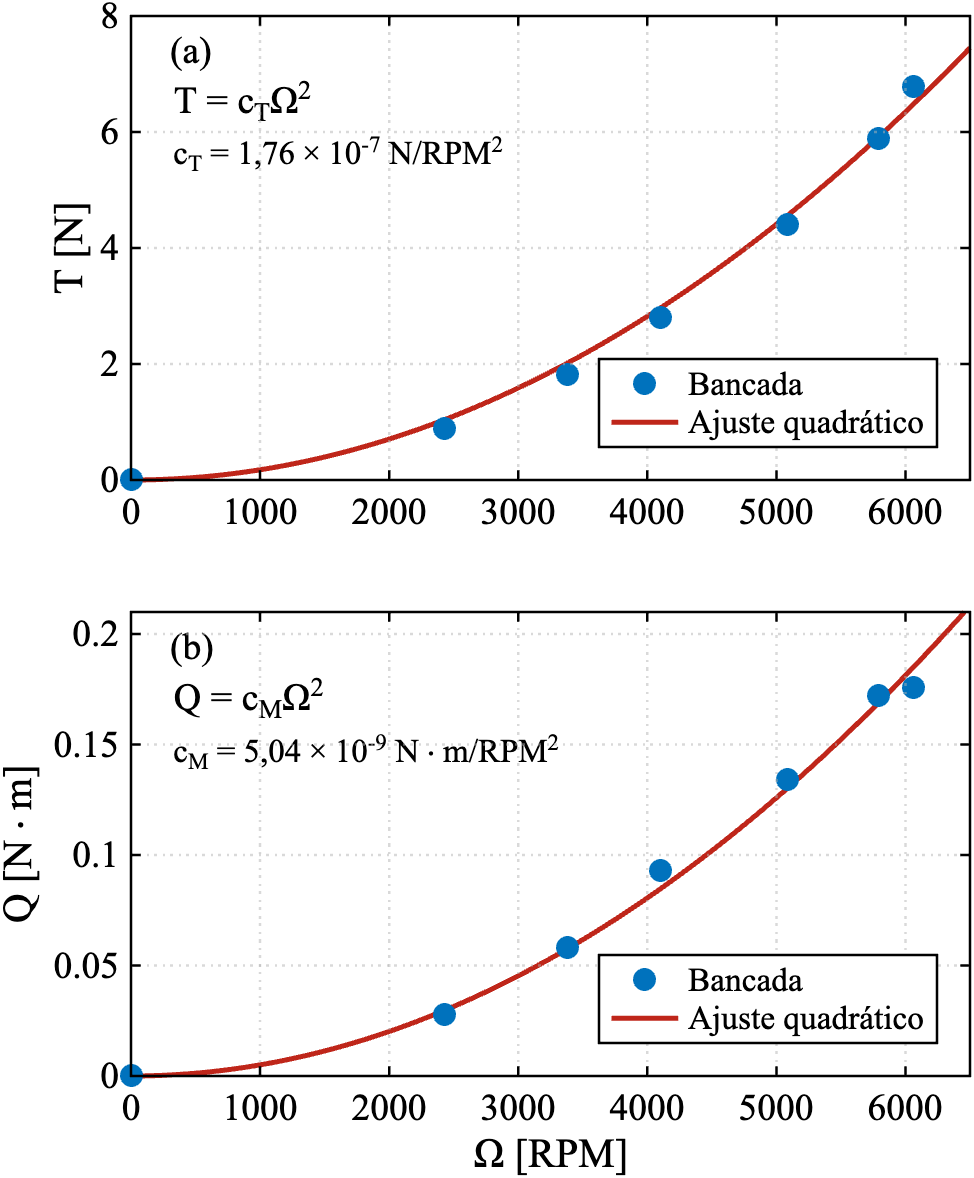
\includegraphics[width=\columnwidth]{motor_thrust_torque.png}
      \caption{Thrust (a) and reaction torque (b) as a function of the rotor angular rate. The points are the bench measurements and the solid lines are the quadratic fits of Equation~\eqref{eq:tq}.}
      \label{fig:motor_tq}
\end{figure}

The individual efforts combine as a function of the aircraft geometry. The roll and pitch moments result from the differential thrust of the motors, weighted by the distances of each rotor to the center of gravity: $L_{x_r}$ and $L_{x_l}$ are the lateral arms of the rotors on the right (motors 1 and 4) and left (motors 2 and 3) sides, and $L_{y_f}$ and $L_{y_r}$ are the longitudinal arms of the front (motors 1 and 3) and rear (motors 2 and 4) rotors, distinct from each other in the H-frame configuration. The yaw moment, in turn, is generated by the reaction torque of the propellers: motors 1 and 2 spin in one direction and motors 3 and 4 in the opposite direction, so as to cancel the resulting torque in hover~\cite{c5}. From Equation~\eqref{eq:tq} the relationship between the reaction torque and the thrust of each rotor is obtained:
\begin{equation}
Q_i = \frac{c_M}{c_T}\,T_i
\label{eq:qt-ratio}
\end{equation}
which allows the reaction torques to be expressed as a function of the thrusts, gathering all contributions into a single allocation matrix $\mathbf{B}$:
\begin{equation}
\begin{bmatrix} T \\ \tau_x \\ \tau_y \\ \tau_z \end{bmatrix}
=
\underbrace{\begin{bmatrix}
1 & 1 & 1 & 1 \\
-L_{x_r} & L_{x_l} & L_{x_l} & -L_{x_r} \\
L_{y_f} & -L_{y_r} & L_{y_f} & -L_{y_r} \\
\tfrac{c_M}{c_T} & \tfrac{c_M}{c_T} & -\tfrac{c_M}{c_T} & -\tfrac{c_M}{c_T}
\end{bmatrix}}_{\mathbf{B}}
\begin{bmatrix} T_1 \\ T_2 \\ T_3 \\ T_4 \end{bmatrix}
\label{eq:aloca}
\end{equation}

The motor model thus establishes the complete path from the bench measurements to the dynamic model: from the PWM--angular-rate pairs $C_R$ is obtained; from the angular-rate--thrust and angular-rate--reaction-torque pairs $c_T$ and $c_M$ are obtained, which generate the thrusts $T_1$ to $T_4$; and the allocation matrix converts these thrusts into the total thrust $T$, which feeds the translational model, and into the moments $\tau_x$, $\tau_y$, and $\tau_z$, which feed the rotational model.

\subsection{Rotational Model}

The rotational model derives from Newton's second law for rotation, which equates the rate of change of the angular momentum $\mathbf{h}$ to the sum of the moments applied to the body $\boldsymbol{\tau}$~\cite{cBeard}:
\begin{equation}
\frac{d\mathbf{h}}{dt} = \boldsymbol{\tau}
\label{eq:rot-newton}
\end{equation}
Expressed in the body frame, with $\mathbf{h} = \mathbf{J}\boldsymbol{\omega}$ and applying the transport theorem, the angular acceleration $\dot{\boldsymbol{\omega}} = [\dot{p}, \dot{q}, \dot{r}]^{\top}$ is isolated in the compact form:
\begin{equation}
\dot{\boldsymbol{\omega}} = \mathbf{J}^{-1}\big[\,\boldsymbol{\tau} - \boldsymbol{\omega} \times (\mathbf{J}\boldsymbol{\omega})\,\big]
\label{eq:rot-compact}
\end{equation}
where $\mathbf{J}$ is the inertia tensor of the rigid body, which relates the angular rates to the angular momenta of the aircraft. For the body frame with origin at the center of gravity, this tensor is given by:
\begin{align}
\mathbf{J} = \begin{bmatrix}
J_{xx} & 0 & -J_{xz} \\
0 & J_{yy} & 0 \\
-J_{xz} & 0 & J_{zz}
\end{bmatrix}
\end{align}
where $J_{xx}$, $J_{yy}$, and $J_{zz}$ are the moments of inertia about the body $x$, $y$, and $z$ axes, respectively, and $J_{xz}$ is the cross product of inertia. The products $J_{xy}$ and $J_{yz}$ are zero due to the symmetry of the $xz$ plane. However, the product of inertia $J_{xz}$ is nonzero, since the aircraft has an H-frame configuration with front and rear arms of distinct lengths, which results in an asymmetric mass distribution with respect to the $xy$ plane. This asymmetry introduces coupling between the roll and yaw axes, making the product $J_{xz}$ a relevant parameter in the modeling and identification of the system.

The expansion of Equation~\eqref{eq:rot-compact} into components uses constants $\Gamma_i$ derived from the aircraft's moments and products of inertia. Defining $\Gamma_0 = J_{xx} J_{zz} - J_{xz}^2$, the constants are:

\begin{align}
\Gamma_1 &= \frac{J_{xz}(J_{xx} - J_{yy} + J_{zz})}{\Gamma_0} \\
\Gamma_2 &= \frac{J_{zz}(J_{zz} - J_{yy}) + J_{xz}^2}{\Gamma_0} \\
\Gamma_3 &= \frac{J_{zz}}{\Gamma_0} \quad , \quad
\Gamma_4 = \frac{J_{xz}}{\Gamma_0} \\
\Gamma_5 &= \frac{J_{zz} - J_{xx}}{J_{yy}} \quad , \quad
\Gamma_6 = \frac{J_{xz}}{J_{yy}} \\
\Gamma_7 &= \frac{J_{xx}(J_{xx} - J_{yy}) + J_{xz}^2}{\Gamma_0} \\
\Gamma_8 &= \frac{J_{xx}}{\Gamma_0}
\end{align}

The angular acceleration equations are then given by:
\begin{align}
\dot{p} &= \Gamma_1 pq - \Gamma_2 qr + \Gamma_3 \tau_x + \Gamma_4 \tau_z - c_p\, p \\
\dot{q} &= \Gamma_5 pr - \Gamma_6 (p^2 - r^2) + \frac{1}{J_{yy}}\tau_y - c_q\, q \\
\dot{r} &= \Gamma_7 pq - \Gamma_1 qr + \Gamma_4 \tau_x + \Gamma_8 \tau_z - c_r\, r
\end{align}

where $\tau_x, \tau_y, \tau_z$ are the control moments generated by the motors, obtained from the allocation matrix (Equation~\eqref{eq:aloca}). The terms $c_p$, $c_q$, and $c_r$ are angular damping coefficients, which model the dissipation of rotational energy due to the aerodynamic drag of the propellers and the fuselage~\cite{c13}. These coefficients are proportional to the angular rate about the respective axis, so that the higher the rotation rate, the greater the damping moment opposing the motion, and they are parameters to be estimated in the identification process, together with the moments of inertia and the motor coefficients.

The equations of the Euler-angle kinematics are:

\begin{align}
\dot{\phi} &= p + \tan\theta(q\sin\phi + r\cos\phi) \\
\dot{\theta} &= q\cos\phi - r\sin\phi \\
\dot{\psi} &= \frac{q\sin\phi + r\cos\phi}{\cos\theta}
\end{align}

\subsection{Translational Model}

The translational model follows from Newton's second law applied to the rigid body, which equates the rate of change of momentum to the sum of the forces $\mathbf{f}$~\cite{cBeard,c11}:
\begin{equation}
m\frac{d\mathbf{v}}{dt} = \mathbf{f}
\label{eq:trans-newton}
\end{equation}
Expressed in the body frame, with $\dot{\mathbf{v}} = [\dot{u}, \dot{v}, \dot{w}]^{\top}$, this relationship becomes:
\begin{equation}
m\big(\dot{\mathbf{v}} + \boldsymbol{\omega} \times \mathbf{v}\big) = \mathbf{f}
\label{eq:trans-compact}
\end{equation}
In quadrotor mode, the only propulsive force is the total thrust $T$, which acts in the negative direction of the body $z$ axis~\cite{c4}:
\begin{equation}
\mathbf{f}_{\text{prop}} = [0,\, 0,\, -T]^{\top}
\label{eq:trans-thrust}
\end{equation}
Gravity, known in the navigation frame as $\mathbf{g}^{n}=[0,\,0,\,g]^{\top}$, is projected into the body frame by the rotation matrix, resulting in the force
\begin{equation}
\mathbf{f}_{g} = m\,\mathbf{g}^{b} = mg\begin{bmatrix} -\sin\theta \\ \sin\phi\cos\theta \\ \cos\phi\cos\theta \end{bmatrix}
\label{eq:trans-grav}
\end{equation}
so that the total force is $\mathbf{f} = \mathbf{f}_{\text{prop}} + \mathbf{f}_{g}$. Considering that, around hover, the translational velocities are small, which allows neglecting the aerodynamic lift and drag of the fixed-wing structure, the translational acceleration equations are given by:

\begin{align}
\dot{u} &= rv - qw - g\sin\theta \\
\dot{v} &= pw - ru + g\sin\phi\cos\theta \\
\dot{w} &= qu - pv + g\cos\phi\cos\theta - \frac{T}{m}
\end{align}

where $T$ is the total thrust obtained from the allocation matrix (Equation~\eqref{eq:aloca}), $g$ is the acceleration of gravity, and $m$ is the total mass of the aircraft.

Since the IMU accelerometer is not mounted at the center of gravity, but offset by a vector $\mathbf{r}_{\mathrm{imu}}$ (Figure~\ref{fig:imu_offset}), it does not measure the specific force of the CG, but rather that of its mounting point. Transporting the specific force of the CG to the sensor position, a tangential term, due to the angular acceleration, and a centripetal term are added~\cite{c3}:
\begin{equation}
\mathbf{a}_{\mathrm{imu}} = \mathbf{a}_{\mathrm{cg}} + \dot{\boldsymbol{\omega}} \times \mathbf{r}_{\mathrm{imu}} + \boldsymbol{\omega} \times (\boldsymbol{\omega} \times \mathbf{r}_{\mathrm{imu}}) + \mathbf{b}
\label{eq:acc-imu}
\end{equation}
where $\boldsymbol{\omega} = [p, q, r]^{\top}$, $\dot{\boldsymbol{\omega}} = [\dot{p}, \dot{q}, \dot{r}]^{\top}$ and $\mathbf{b}$ is the constant bias of the sensor. Since this coupling brings the angular rates and accelerations into the accelerometer reading, the signal carries information about the rotational dynamics, exploited in the parameter estimation.

Gathering the rotational and translational dynamics, the model of the quadrotor mode is written compactly as the nonlinear state-space system $\dot{x} = f(x, u, \Theta)$, with the state vector $x$ and the inputs $u$ defined previously. The vector $\Theta$ gathers the physical parameters to be identified: the moments and the product of inertia, the thrust and reaction-torque coefficients of each motor, and the rotational damping coefficients:
\begin{equation}
\begin{aligned}
\Theta = [\,&J_{xx},\,J_{yy},\,J_{zz},\,J_{xz},\;c_{T_1},\dots,c_{T_4},\\
&c_{M_1},\dots,c_{M_4},\;c_p,\,c_q,\,c_r\,]^{\top}
\end{aligned}
\label{eq:theta}
\end{equation}
Therefore, for the determination of $\Theta$, estimation methods are used so that the simulated response of the model reproduces the obtained measurements, which is the subject of the following section.

\section{Parameter Estimation}
\label{sec:estimacao}

The estimation of the parameters of the quadrotor-mode model combines two complementary time-domain methods: the Equation-Error Method (EEM), which provides an initial algebraic estimate, and the Output-Error Method (OEM), which refines it by maximum likelihood~\cite{c2}. Both seek the parameter vector $\Theta$ (Equation~\eqref{eq:theta}) that minimizes the residuals between the measured outputs $z(t_k)$ and those simulated by the model $y(t_k,\Theta)$.

The coefficients $c_{T_i}$ and $c_{M_i}$ start from the bench values and are refined individually for each motor, just as the moments and the product of inertia start from the values obtained by simulating the three-dimensional model of the aircraft, all these parameters being refined in the estimation. The identification begins in the rotational subsystem, because since the angular acceleration equations of the rotational model are isolated in the angular-rate variables, it suffices to integrate this subsystem, fed by the moments reconstructed from the PWM commands by the motor model and the allocation matrix (Equation~\eqref{eq:aloca}); the translational model is then introduced in the OEM method with the measured angular rates, simulated attitudes, and comparing the specific forces of the accelerometer.

\subsection{Equation-Error Method (EEM)}

Initially, with the initial value $\Theta_0$, the EEM method is applied using the measured values of $p$, $q$, and $r$ to feed the model back at all time instants of the identification window, which dispenses with the numerical integration of the model, since the dynamic equation is evaluated directly on the measured states and their derivatives, the latter being computed by numerical differentiation of the measured angular rate. The equation residual is defined as the difference between the angular-rate derivative and that predicted by the moment equations of the rotational model with the initial parameters and measured angular-rate values:
\begin{equation}
e_{\text{EEM}}(t_k) = \dot{\omega}_{\text{med}}(t_k) - f_\omega\big(\omega_{\text{med}}(t_k),\, \tau(t_k),\, \Theta_0\big)
\label{eq:eem-res}
\end{equation}
with $\omega_{med} = [p_{med}, q_{med}, r_{med}]^{\top}$. The parameters are obtained by minimizing the weighted squared error over the concatenated training segments:
\begin{equation}
\Theta_{\text{EEM}} = \arg\min_{\Theta} \sum_{k} \big\| \mathbf{W}_e^{1/2}\, e_{\text{EEM}}(t_k) \big\|^2
\label{eq:eem-cost}
\end{equation}
where $\mathbf{W}_e = \mathrm{diag}(1/\sigma_i^2)$ is the diagonal weight matrix that acts on the three rotational channels of the equation residual $(\dot{p},\dot{q},\dot{r})$, weighting each by the inverse of its variance, and $\dot{\omega}_{\text{med}}$ is obtained by numerical differentiation of the smoothed signal. With the inertias fixed at their initial values, the residual of Equation~\eqref{eq:eem-res} is linear in the motor and damping coefficients, making Equation~\eqref{eq:eem-cost} a least-squares problem with a fast and robust solution. On the other hand, the use of the measured derivatives, which amplify the noise, introduces bias, which is why the EEM serves as a starting point and not as a final estimate~\cite{c2}.

\subsection{Output-Error Method (OEM)}

The OEM aims to eliminate the bias introduced in the previous stage, by comparing the integrated output of the model with the measurements iteratively as the parameters are refined. Starting from $\Theta_{\text{EEM}}$, the rotational subsystem is integrated in time (4th-order Runge--Kutta) with the same input applied to the vehicle, producing the simulated output $y(t_k, \Theta)$, resulting in the residual that is the output error $z(t_k) - y(t_k, \Theta)$.

The outputs gather the angular rates $(p, q, r)$ and the specific forces measured by the IMU $(a_x, a_y, a_z)$, and the weighting by $\mathbf{W}$, now diagonal over these six output channels (distinct from $\mathbf{W}_e$, which acts on the equation residual), normalizes the different quantities (rad/s vs.\ m/s$^2$), preventing the channels of larger magnitude from dominating the fit. Figure~\ref{fig:oem_schematic} summarizes the general scheme of the method, whose iterative cycle is detailed later in Figure~\ref{fig:opt_loop}.

Under the assumption of Gaussian measurement noise with covariance $\mathbf{R}_\nu$, the OEM is a maximum-likelihood estimator, which minimizes the cost~\cite{c2}:
\begin{equation}
J(\Theta) = \frac{1}{2} \sum_{k=1}^{N} \big[z(t_k) - y(t_k,\Theta)\big]^{\top} \mathbf{R}_\nu^{-1} \big[z(t_k) - y(t_k,\Theta)\big]
\label{eq:oem-cost}
\end{equation}
The minimum is sought by the Gauss--Newton method: linearizing the output around the current estimate, $y(\Theta + \delta) \approx y(\Theta) + S\,\delta$, with the sensitivity matrix
\begin{equation}
S(t_k) = \frac{\partial y(t_k, \Theta)}{\partial \Theta}
\label{eq:sens}
\end{equation}
the step $\delta$ that nullifies the gradient of the cost solves the normal equations
\begin{equation}
\Big[\textstyle\sum_{k} S_k^{\top} \mathbf{R}_\nu^{-1} S_k\Big]\, \delta = \textstyle\sum_{k} S_k^{\top} \mathbf{R}_\nu^{-1}\big(z(t_k) - y(t_k,\Theta)\big)
\label{eq:gauss-newton}
\end{equation}
whose bracketed term is the Fisher information matrix $F$. The parameters are then updated by:
\begin{equation}
\Theta_{j+1} = \Theta_{j} + \delta
\label{eq:update}
\end{equation}
\begin{figure}[!t]
\centering
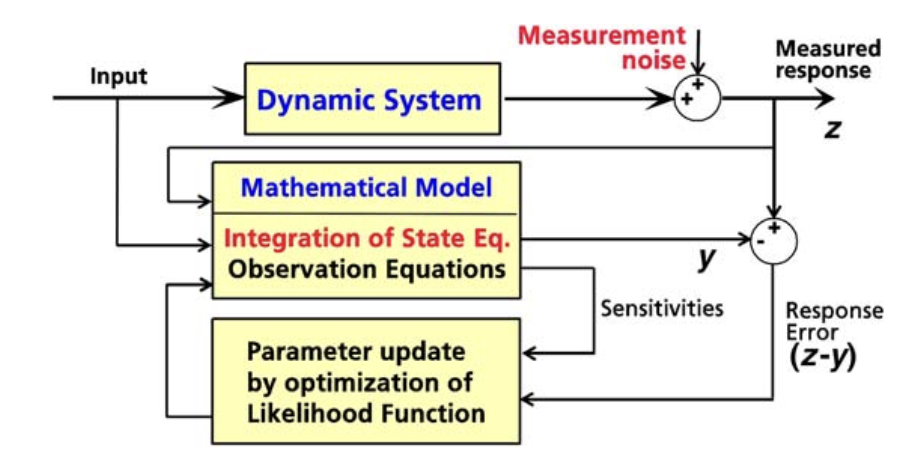
\includegraphics[width=\columnwidth]{images/intro-oem.png}
\caption{General scheme of the output-error method. Adapted from~\cite{c2}.}
\label{fig:oem_schematic}
\end{figure}

\begin{figure}[!t]
\centering
\resizebox{\columnwidth}{!}{%
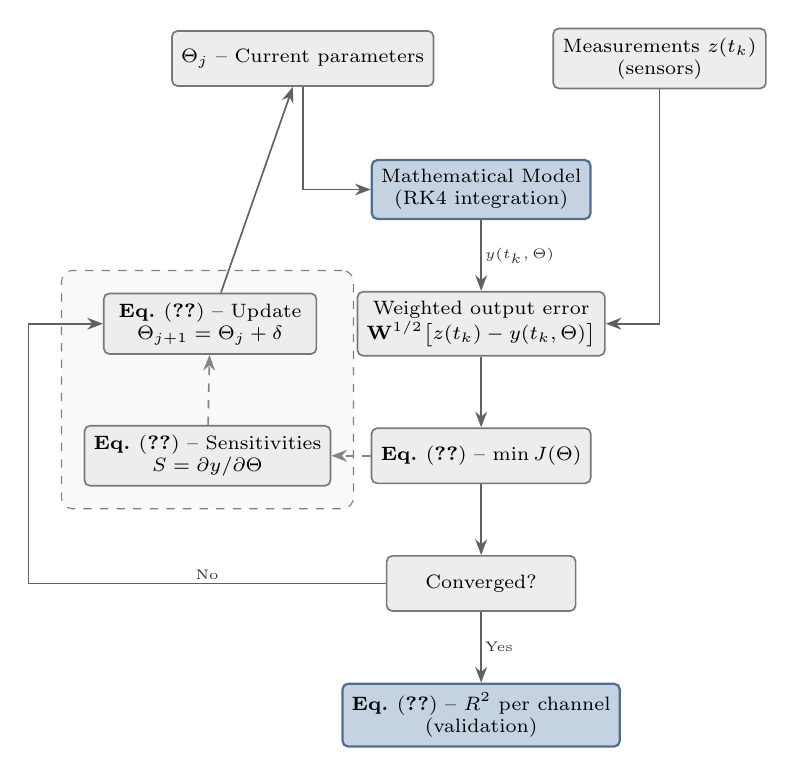
\begin{tikzpicture}[
    node distance=0.9cm,
    block/.style={rectangle, draw=blkEdge, semithick, rounded corners=2pt, minimum width=2.7cm, minimum height=0.7cm, align=center, font=\scriptsize},
    decis/.style={rectangle, draw=blkEdge, semithick, rounded corners=2pt, fill=blkBase, minimum width=2.4cm, minimum height=0.7cm, align=center, font=\scriptsize},
    hi/.style={fill=blkHi, draw=blkHiEdge, thick},
    arrow/.style={-{Stealth[length=2mm]}, semithick, black!62},
    dasharrow/.style={-{Stealth[length=2mm]}, semithick, dashed, black!48},
    lbl/.style={font=\tiny, fill=white, inner sep=1pt, text=black!80}
]

% --- Top: Parameters (left) and Measurements (right) ---
\node[block, fill=blkBase] (theta)
    {$\Theta_j$ -- Current parameters};

\node[block, fill=blkBase, right=1.5cm of theta] (data)
    {Measurements $z(t_k)$\\(sensors)};

% --- Central column (between theta and data) ---
\node[block, hi, below=0.9cm of $(theta.south)!0.5!(data.south)$] (model)
    {Mathematical Model\\(RK4 integration)};

\node[block, fill=blkBase, below=of model] (resid)
    {Weighted output error\\$\mathbf{W}^{1/2}\big[z(t_k) - y(t_k,\Theta)\big]$};

\node[block, fill=blkBase, below=of resid] (lsq)
    {\textbf{Eq.~\eqref{eq:oem-cost}} -- $\min J(\Theta)$};

\node[decis, below=of lsq] (conv) {Converged?};

\node[block, hi, below=of conv] (r2)
    {\textbf{Eq.~\eqref{eq:r2}} -- $R^2$ per channel\\(validation)};

% --- Left: lsqnonlin internal ---
\node[block, fill=blkBase, left=0.5cm of lsq] (jac)
    {\textbf{Eq.~\eqref{eq:sens}} -- Sensitivities\\$S = \partial y / \partial \Theta$};

\node[block, fill=blkBase, left=0.5cm of resid] (update)
    {\textbf{Eq.~\eqref{eq:update}} -- Update\\$\Theta_{j+1} = \Theta_j + \delta$};

% === SETAS ===
\draw[arrow] (theta) |- (model);
\draw[arrow] (model) -- node[lbl, right] {$y(t_k,\Theta)$} (resid);
\draw[arrow] (resid) -- (lsq);
\draw[arrow] (lsq) -- (conv);
\draw[arrow] (conv) -- node[lbl, right] {Yes} (r2);

% Data -> residuals (comes down from the top)
\draw[arrow] (data) |- (resid);

% lsqnonlin internal
\draw[dasharrow] (lsq) -- (jac);
\draw[dasharrow] (jac) -- (update);

% No -> update (routes around the left side)
\coordinate (aux) at ([xshift=-0.7cm]jac.west);
\draw[arrow] (conv.west) -| node[lbl, near start, above] {No} (aux) |- (update.west);

% Loop back
\draw[arrow] (update) -- (theta);

% Dashed box
\begin{scope}[on background layer]
\node[draw=gray, dashed, rounded corners=4pt, fill=gray!5,
      inner xsep=8pt, inner ysep=8pt,
      fit=(jac)(update),
      label={[font=\tiny, text=gray]above: }] {};
\end{scope}

\end{tikzpicture}%
}
\caption{Iterative cycle of the output-error method. Adapted from~\cite{c2}.}
\label{fig:opt_loop}
\end{figure}

The cycle of integrating the model to form the output error, computing the sensitivities, and updating the parameters repeats until convergence, as illustrated in Figure~\ref{fig:opt_loop}. In the implementation, the sensitivities are computed by finite differences, the inverse covariance $\mathbf{R}_\nu^{-1}$ is approximated by the fixed diagonal weight matrix $\mathbf{W} = \mathrm{diag}(1/\sigma_i^2)$, whose elements are the inverse of the variance of each output channel, and the step $\delta$ is determined by the \textit{Trust-Region Reflective} algorithm~\cite{c2} of MATLAB's \texttt{lsqnonlin} function, which globalizes the Gauss--Newton and imposes the physical bounds of the parameters.

The quality of the fit is evaluated by the coefficient of determination, computed for each output channel on a validation segment that does not participate in the optimization:
\begin{equation}
R^2 = 1 - \frac{\sum_{k}(z_k - y_k)^2}{\sum_{k}(z_k - \bar{z})^2}
\label{eq:r2}
\end{equation}
where $\bar{z}$ is the mean of the measurements, and values close to 1 indicate a good agreement between model and data. At convergence, the inverse of the Fisher information matrix $F$ (Equation~\eqref{eq:gauss-newton}) provides the covariance of the estimates (Cramér--Rao bound), from which the relative standard deviation of each parameter is extracted; high values signal parameters poorly observable from the data~\cite{c2}.

\subsection{Multi-Window Output-Error Method}

In this work, the parameter estimation was carried out by means of the Output-Error Method (OEM) with a progressive multi-window strategy. Unlike the conventional OEM, which integrates the model over the entire flight record with a single initial condition, the multi-window approach divides each data segment into smaller time windows. At the beginning of each window, the model states are reinitialized with the measured values, so that integration errors do not propagate between adjacent windows. This significantly increases the robustness of the identification, since it prevents local divergences from contaminating the rest of the simulation.

The identification process is divided into two sequential phases, as illustrated in Figure~\ref{fig:oem_diagram}:

\begin{itemize}
    \item \textbf{Phase A -- EEM (Equation-Error Method):} The data of all training segments are concatenated and used in an algebraic formulation (without numerical integration). The rotational parameters are estimated by minimizing the error between the measured angular derivatives and those computed by the model. This phase provides a robust initial estimate $\Theta_{\text{EEM}}$ for Phase B.
    \item \textbf{Phase B -- Progressive OEM (Output-Error Method):} Using the values of $\Theta_{\text{EEM}}$ as the initial values of $\Theta$, the model is integrated numerically with RK4 within each window. The window duration is progressively increased, so that in the early stages the optimizer adjusts the parameters with a lower risk of divergence. At each stage, the performance is evaluated on the validation segment, and the parameter set with the best coefficient of determination $R^2$ is selected as the final result $\Theta_{\text{OEM}}$.
\end{itemize}

The cost function is the same as that of the OEM (Equation~\eqref{eq:oem-cost}, with $\mathbf{R}_\nu^{-1} \approx \mathbf{W}$), now aggregating the weighted residuals of all windows of all training segments:
\begin{align}
J(\Theta) = \sum_{s=1}^{N_s} \sum_{w=1}^{N_w^{(s)}} \sum_{k \in \mathcal{W}_w^{(s)}} \left\| \mathbf{W}^{1/2} \left[ z(t_k) - y(t_k, \Theta) \right] \right\|^2
\end{align}
where $N_s$ is the number of training segments, $N_w^{(s)}$ is the number of windows in segment $s$, $\mathcal{W}_w^{(s)}$ are the time indices of window $w$, and $\mathbf{W}^{1/2}$ is the square root of the weight matrix as defined previously. The outputs $z$ and $y$ include both the angular rates $(p, q, r)$ and the specific forces measured by the IMU $(a_x, a_y, a_z)$.

\begin{figure}[!htbp]
\centering
\resizebox{\columnwidth}{!}{%
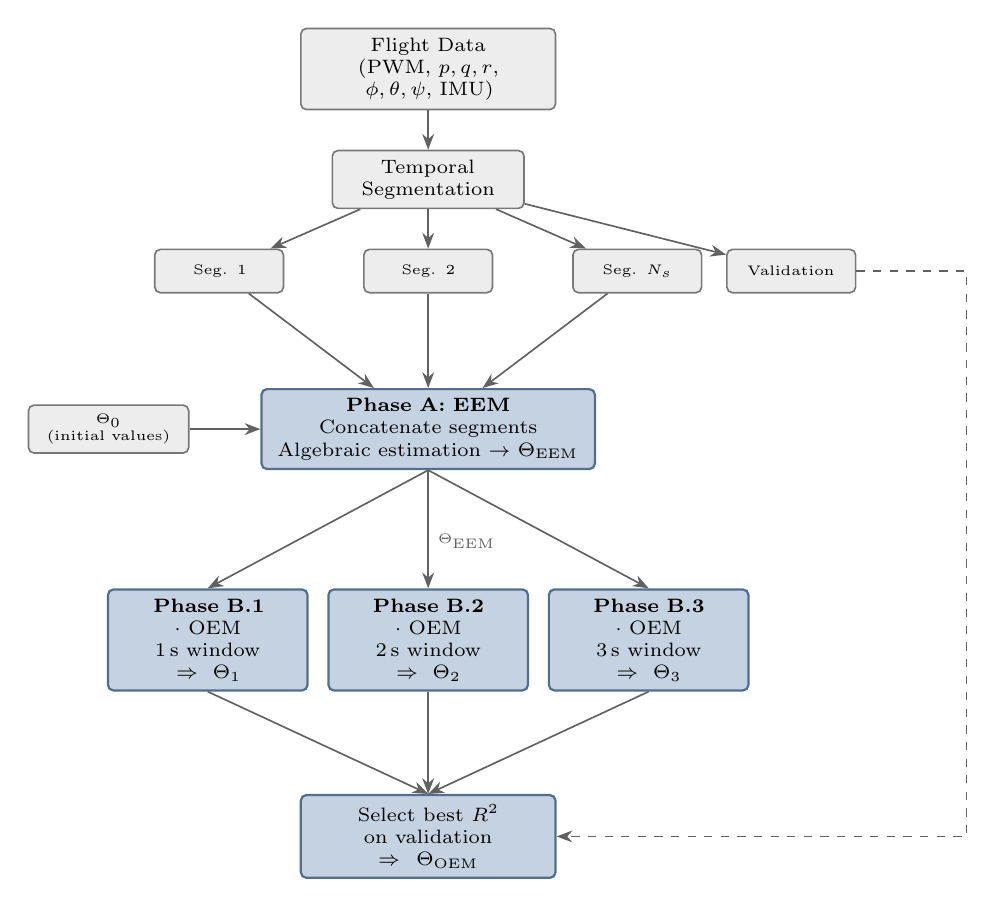
\begin{tikzpicture}[
    node distance=0.6cm and 0.4cm,
    block/.style={rectangle, draw=blkEdge, semithick, rounded corners=2pt, fill=blkBase, text width=2.2cm, minimum height=0.7cm, align=center, font=\scriptsize},
    bigblock/.style={rectangle, draw=blkEdge, semithick, rounded corners=2pt, fill=blkBase, text width=2.8cm, minimum height=0.7cm, align=center, font=\scriptsize},
    smallblock/.style={rectangle, draw=blkEdge, semithick, rounded corners=2pt, fill=blkBase, text width=1.4cm, minimum height=0.55cm, align=center, font=\tiny},
    hi/.style={fill=blkHi, draw=blkHiEdge, thick},
    arrow/.style={-{Stealth[length=2mm]}, semithick, black!62},
    every node/.style={font=\scriptsize}
]

% Top: Flight Data
\node[block, fill=blkBase, text width=3cm] (data) {Flight Data\\(PWM, $p,q,r$, $\phi,\theta,\psi$, IMU)};

% Segmentation
\node[block, below=0.5cm of data] (seg) {Temporal Segmentation};

% Segments
\node[smallblock, below left=0.5cm and 0.6cm of seg] (s1) {Seg. 1};
\node[smallblock, below=0.5cm of seg] (s2) {Seg. 2};
\node[smallblock, below right=0.5cm and 0.6cm of seg] (sn) {Seg. $N_s$};
\node[smallblock, right=0.3cm of sn, fill=blkBase] (val) {Validation};

% Phase A
\node[bigblock, below=1.2cm of s2, hi, text width=4cm] (eembox) {\textbf{Phase A: EEM}\\Concatenate segments\\Algebraic estimation $\to \Theta_{\text{EEM}}$};

% Initial parameters
\node[smallblock, left=0.9cm of eembox, text width=1.8cm] (theta0) {$\Theta_0$\\(initial values)};

% Phase B: OEM in three windows, all starting from the same Theta_EEM (parallel)
\node[block, below=1.5cm of eembox, hi, xshift=-2.8cm, text width=2.3cm] (b1) {\textbf{Phase B.1} $\cdot$ OEM\\1\,s window\\$\Rightarrow \Theta_1$};
\node[block, below=1.5cm of eembox, hi, text width=2.3cm] (b2) {\textbf{Phase B.2} $\cdot$ OEM\\2\,s window\\$\Rightarrow \Theta_2$};
\node[block, below=1.5cm of eembox, hi, xshift=2.8cm, text width=2.3cm] (b3) {\textbf{Phase B.3} $\cdot$ OEM\\3\,s window\\$\Rightarrow \Theta_3$};

% Best selection (below the row)
\node[block, below=1.3cm of b2, hi, text width=3.0cm] (best) {Select best $R^2$ on validation\\$\Rightarrow \Theta_{\text{OEM}}$};

% Arrows
\draw[arrow] (data) -- (seg);
\draw[arrow] (seg) -- (s1);
\draw[arrow] (seg) -- (s2);
\draw[arrow] (seg) -- (sn);
\draw[arrow] (seg) -- (val);

\draw[arrow] (s1) -- (eembox);
\draw[arrow] (s2) -- (eembox);
\draw[arrow] (sn) -- (eembox);
\draw[arrow] (theta0) -- (eembox);

% The same Theta_EEM feeds the three stages (parallel)
\draw[arrow] (eembox.south) -- (b1.north);
\draw[arrow] (eembox.south) -- node[pos=0.6, right, font=\tiny] {$\Theta_{\text{EEM}}$} (b2.north);
\draw[arrow] (eembox.south) -- (b3.north);

% Each stage generates a candidate -> selection
\draw[arrow] (b1.south) -- (best.north);
\draw[arrow] (b2.south) -- (best.north);
\draw[arrow] (b3.south) -- (best.north);

% Validation (dashed), set apart from the blocks
\draw[arrow, dashed] (val.east) -- ++(1.4,0) |- (best.east);

\end{tikzpicture}%
}
\caption{Diagram of the identification process. Starting from the initial values {\mathversion{normal}$\Theta_0$}, Phase~A (algebraic EEM) provides {\mathversion{normal}$\Theta_{\text{EEM}}$}, which feeds Phase~B: the OEM is executed and returns a {\mathversion{normal}$\Theta_{OEM}$}.}
\label{fig:oem_diagram}
\end{figure}

The reinitialization of the states at the beginning of each window is a fundamental aspect of the approach. Within each window $w$, the RK4 integrator starts from the measured initial conditions $z(t_{w,0})$ and propagates the states to the end of the window. This technique, known as \textit{multiple shooting}, ensures that the error of each window depends only on the local quality of the parameters, and not on the accumulation of errors from previous windows.

\section{Methodology}
\label{sec:metodologia}

The methodological approach of this work is grounded in the M4V system identification framework. The practical steps involved the collection of flight data in quadrotor mode through specific maneuvers, the determination of initial constants for the model, and the implementation of the mathematical model in a simulation environment for the identification process.

\subsection{Maneuvers and Data for Identification}

The quality of the identification depends directly on the richness of the collected data. To ensure sufficient excitation of the quadrotor-mode dynamics, flight maneuvers were performed, designed to excite the motion modes about the principal axes: roll, pitch, and yaw~\cite{c7},~\cite{c8}. All maneuvers were performed with the aircraft operating exclusively in quadrotor mode, with the cruise motor turned off.

The maneuvers adopted were of the \textit{doublet} type, applied to one axis at a time, in which the command is abruptly shifted in one direction, held for an interval $\Delta t_{\text{db}}$, reversed for an equal interval, and returned to neutral. Being symmetric, the \textit{doublet} concentrates the excitation energy in the band around the characteristic frequency $\omega_n$ of the channel to be identified, with practically zero energy at zero frequency, which allows the pulse width to be sized by $\Delta t_{\text{db}} \approx 2.3/\omega_n$~\cite{c2},~\cite{c3}. In the pilot commands (RCIN) of Figure~\ref{fig:exc_dataset}, the roll and pitch \textit{doublets} have a width $\Delta t_{\text{db}} \approx 0.4$~s and energy concentrated near $1$~Hz, within the band of the rate dynamics. Yaw, in turn, with lower control authority and a slower response, did not allow the same variation, resulting in a \textit{doublet} motion about five times slower ($\Delta t_{\text{db}} \approx 2.0$~s), with energy around $0.23$~Hz.

The onboard instrumentation is centered on the Pixhawk 2.4.0 (3DR) flight controller, which runs the ArduPilot \textit{firmware} and logs all flight signals, from the radio commands to the PWM outputs and the sensor measurements. The inertial quantities come from the IMU integrated into the controller, an InvenSense MPU-6000 sensor that combines a three-axis accelerometer and gyroscope sampled at about $25$~Hz: the gyroscope provides the angular rates $(p, q, r)$ and the accelerometer the specific forces $(a_x, a_y, a_z)$. The attitude is not measured directly, but estimated by the controller's EKF from the gyroscope, accelerometer, and magnetometer, with the positioning supported by a u-blox M8 GPS receiver.

The data were extracted directly from the aircraft's flight logs~\cite{c9}. Since the controller's sensors record at distinct rates and instants, all channels were synchronized by interpolation onto a common time grid of $10$~Hz ($\Delta t = 0.1$~s); as the rate dynamics of the quadrotor is concentrated below $2$~Hz, this rate is about five times the band of interest, which represents the dynamics without loss of information. Subsequently, a Savitzky--Golay digital filter was applied to suppress the high-frequency noise, especially the motor vibration; being symmetric, it introduces no phase delay and is applied equally to the input and the output, preserving the input--output relationship.

The complete flight campaign, already resampled and filtered, is presented in Figure~\ref{fig:exc_dataset}, whose panels gather, from top to bottom, the pilot command (RCIN), the motor PWM command, the angular rates ($p, q, r$), and the accelerometer specific forces ($a_x, a_y, a_z$). The data were separated into two groups of windows. The training windows (in green), $\Delta T_1$, $\Delta T_2$, and $\Delta T_3$, which isolate one axis at a time, separately exciting roll, pitch, and yaw, which makes the dynamics of each channel identifiable independently. The validation windows (in orange), $\Delta T_4$ and $\Delta T_5$, which contain compound motion, with the three axes excited simultaneously, allowing the model to be evaluated under conditions distinct from those of training and avoiding overfitting to a single axis.

\begin{figure}[!htbp]
      \centering
      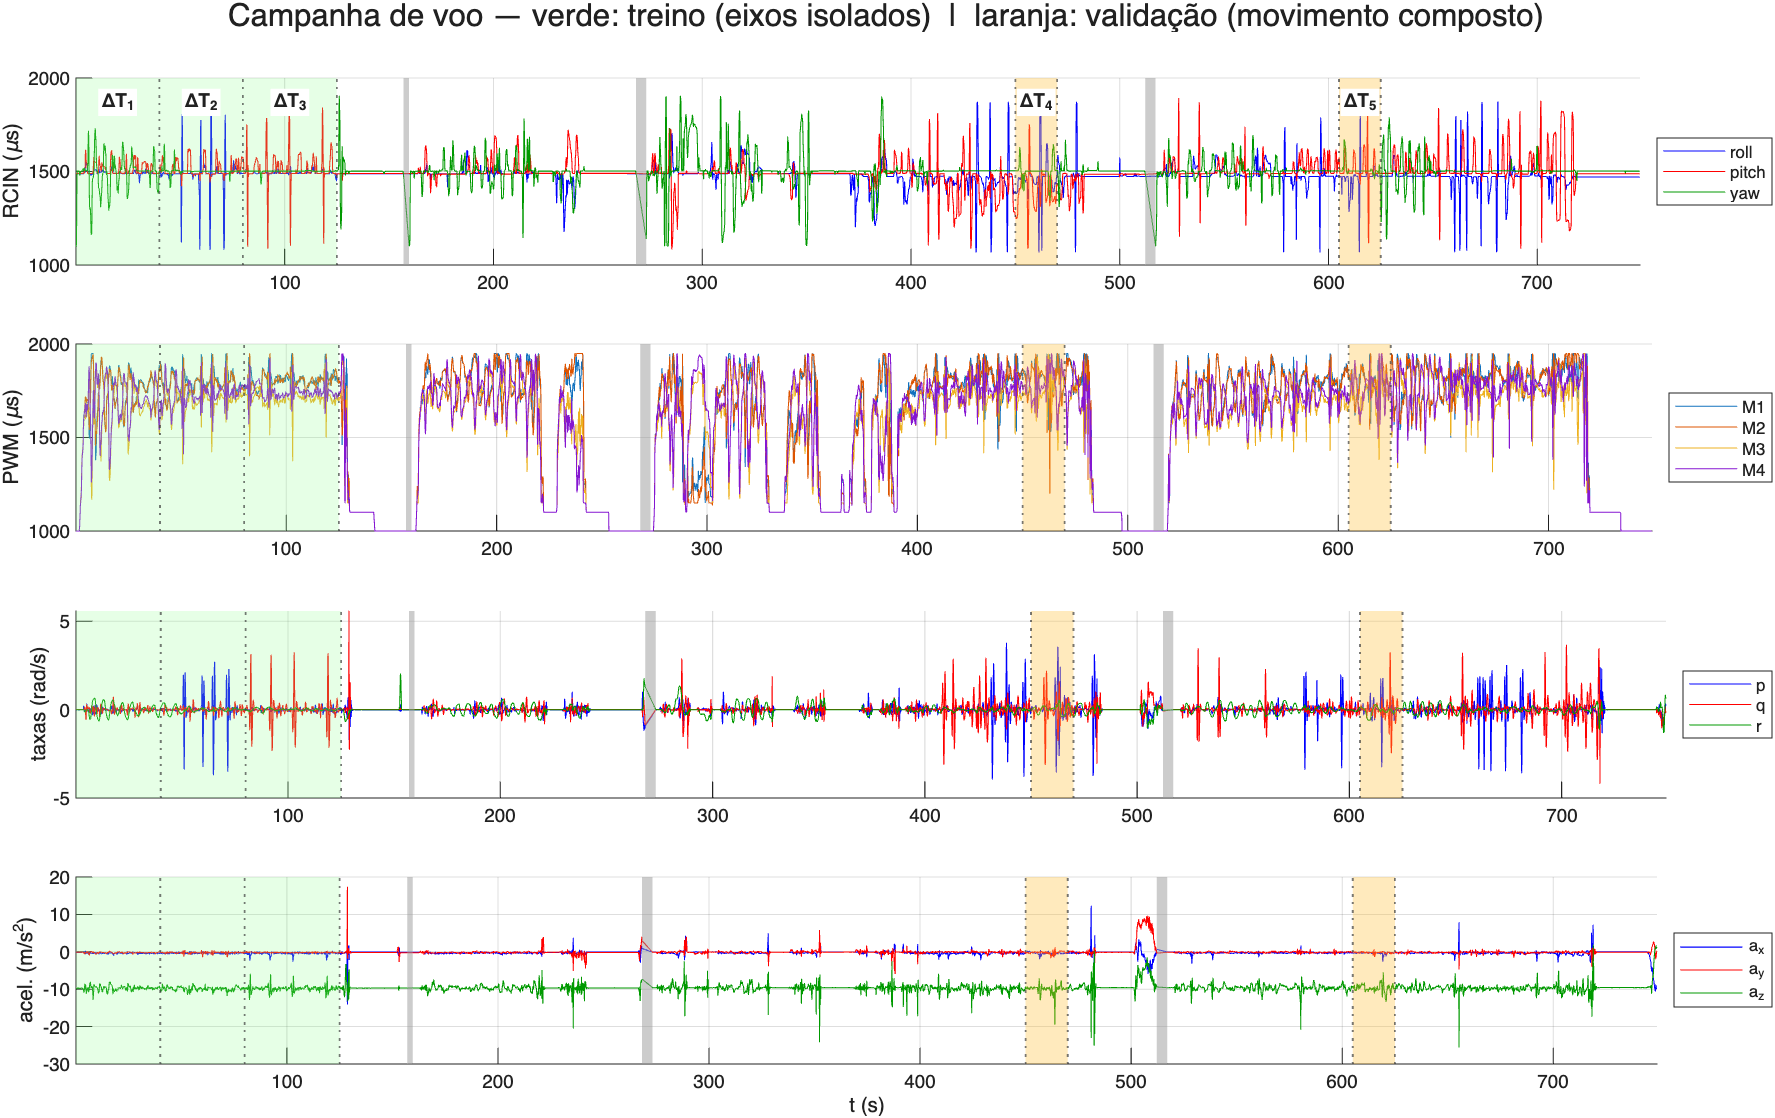
\includegraphics[width=\columnwidth]{exc_dataset.png}
      \caption{Complete flight campaign: in green, the training windows ($\Delta T_1$--$\Delta T_3$, isolated axes); in orange, the validation windows ($\Delta T_4$, $\Delta T_5$, compound motion).}
      \label{fig:exc_dataset}
\end{figure}

Figure~\ref{fig:exc_overview} details this signal chain in representative identification segments of the flight: the pilot command (RCIN) is converted into the PWM actually sent to the motors (RCOU), which forms the input $u$, which generates the control moments reconstructed by the allocation matrix ($\tau_x, \tau_y, \tau_z$) and, finally, the response angular rates ($p, q, r$), highlighting the chaining between the command and the aircraft response that the identification seeks to reproduce.

\begin{figure}[!htbp]
      \centering
      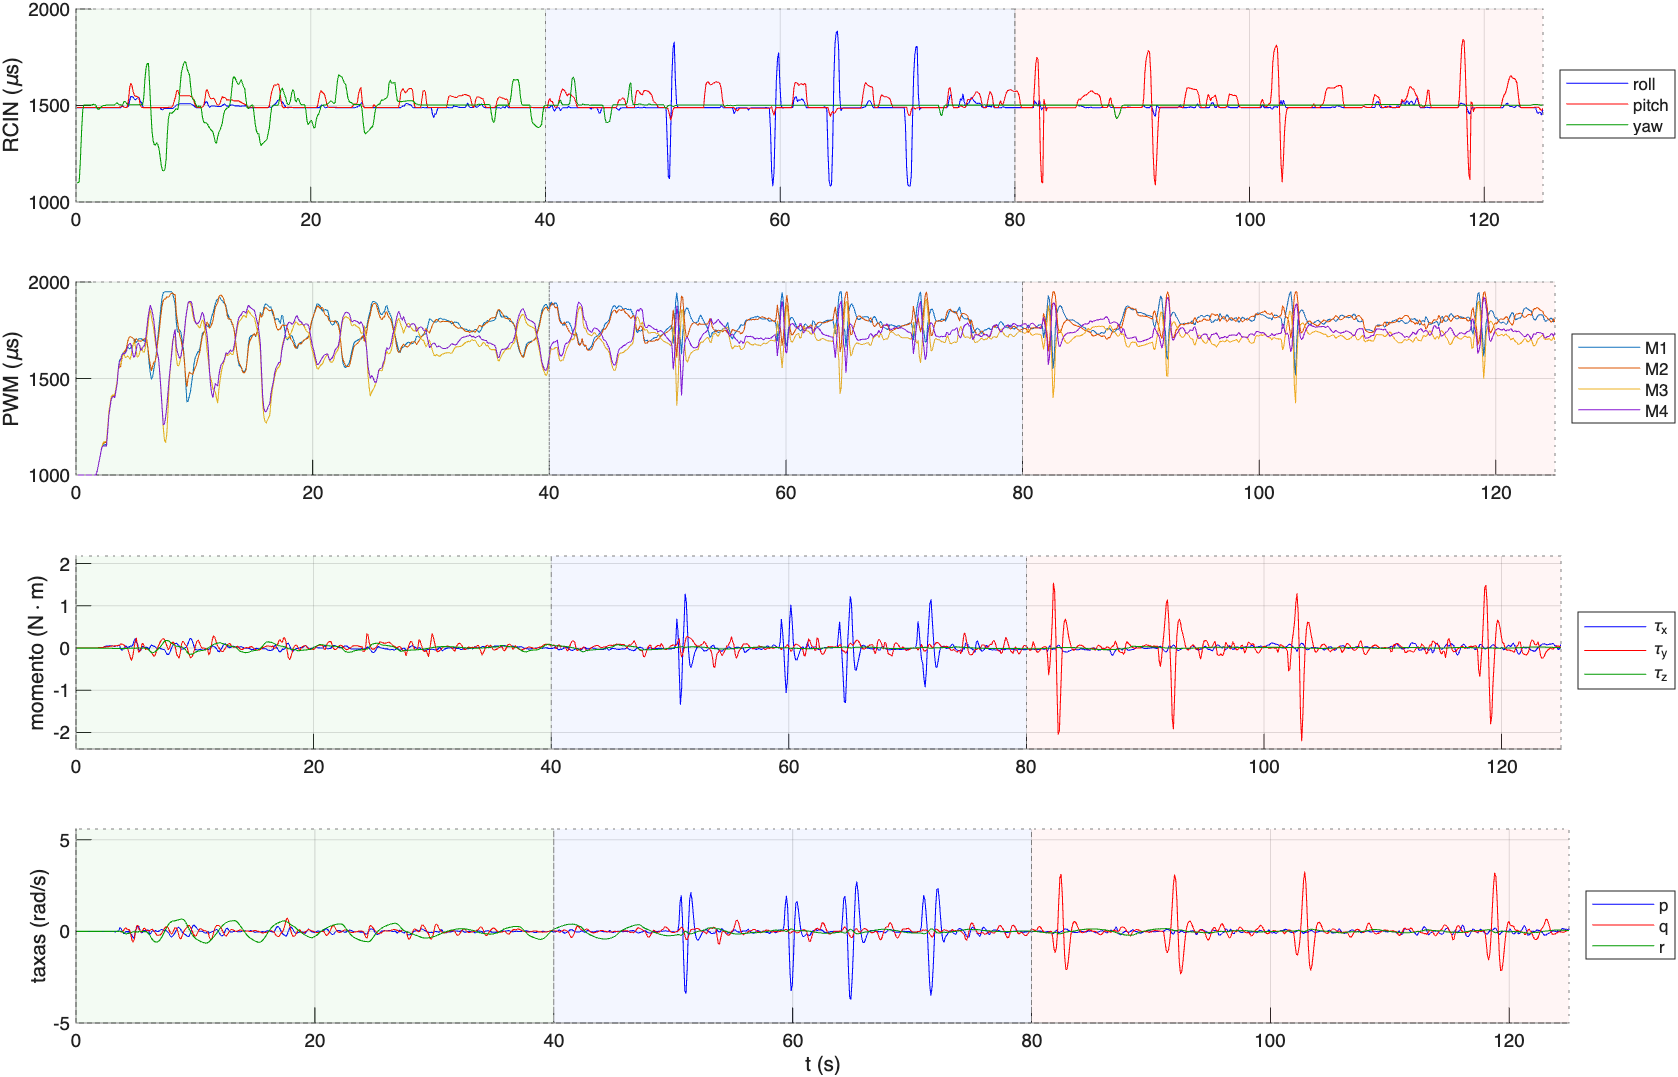
\includegraphics[width=\columnwidth]{exc_overview.png}
      \caption{Signal chain of the excitation in a flight segment: pilot command (RCIN), motor PWM (RCOU), generated moments ($\tau_x, \tau_y, \tau_z$), and response angular rates ($p, q, r$).}
      \label{fig:exc_overview}
\end{figure}



\pagebreak
In each window, the identification relates the input and the output of the system:
\begin{sloppypar}
\begin{itemize}
    \item \textbf{Input ($u$):} the Pulse-Width Modulation (PWM) signals sent to the four vertical motors;
    \item \textbf{Output ($y$):} the angular rates in the body frame, roll ($p$), pitch ($q$), and yaw ($r$), as well as the specific forces measured by the IMU ($a_x$, $a_y$, $a_z$), in rad/s and m/s$^2$, respectively.
\end{itemize}
\end{sloppypar}

\subsection{Fixed Model Constants}
\begin{sloppypar}
The initial constants of the model were obtained through physical measurements of the aircraft and the bench tests of the motor model. The distances between each rotor and the center of gravity, which define the moment arms of the allocation matrix, are presented in Figure~\ref{fig:bracos}, and the main initial values are gathered in Table~\ref{tab:const_iniciais}.
\end{sloppypar}

\begin{figure}[!htbp]
      \centering
      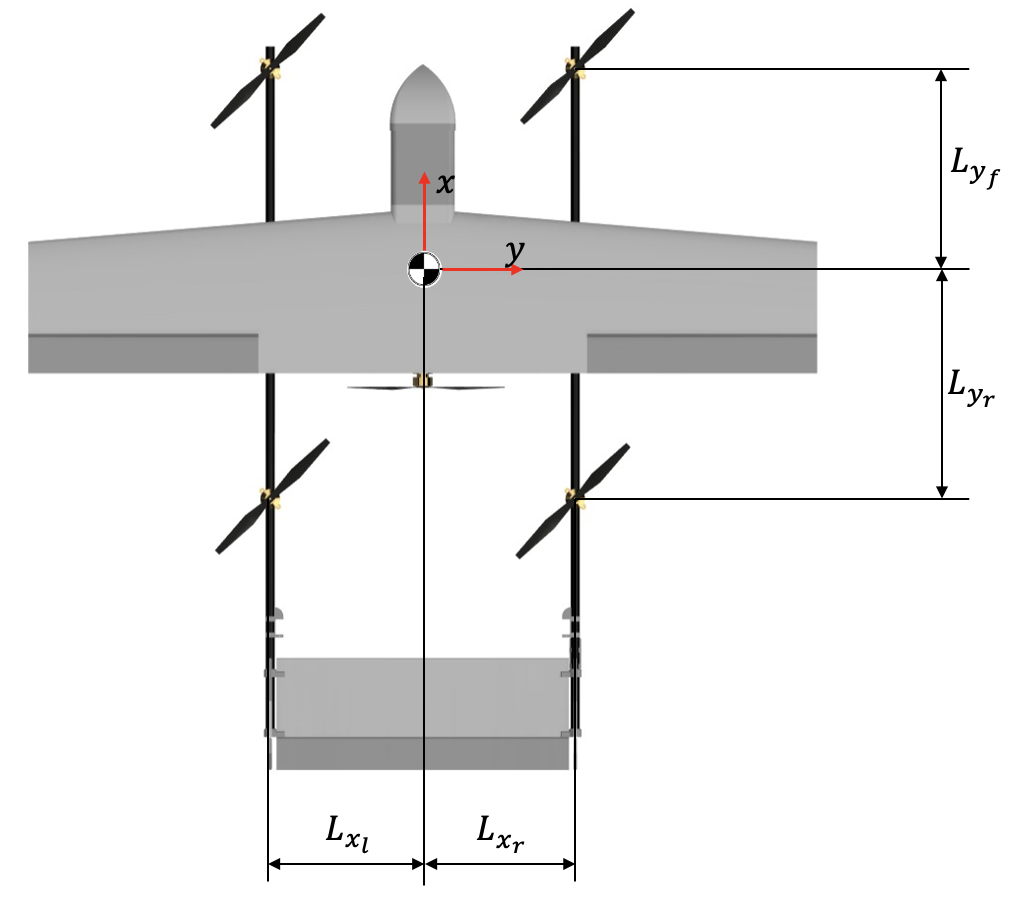
\includegraphics[width=0.8\columnwidth]{bracos.png}
      \caption{Distances between the motors and the CG.}
      \label{fig:bracos}
\end{figure}

\begin{table*}[!htbp]
\caption{Fixed model constants.}
\label{tab:const_iniciais}
\centering
\begin{tabular}{llccl}
\toprule
\textbf{Constant} & \textbf{Description} & \textbf{Value} & \textbf{Unit} & \textbf{Source} \\
\midrule
$L_{x_l} = L_{x_r}$ & Lateral arm from CG to rotors (left and right) & 0.232 & m & Physical measurement \\
$L_{y_f}$ & Longitudinal arm from CG to front rotors & 0.330 & m & Physical measurement \\
$L_{y_r}$ & Longitudinal arm from CG to rear rotors & 0.323 & m & Physical measurement \\
$r_{\mathrm{imu}_x}$ & Longitudinal offset of the IMU relative to the CG & 0.10 & m & Physical measurement \\
$r_{\mathrm{imu}_z}$ & Vertical offset of the IMU relative to the CG & 0.02 & m & Physical measurement \\
$c_{T_0}$ & Initial rotor thrust coefficient & $1.76\times10^{-7}$ & N/RPM$^2$ & Bench test \\
$c_{M_0}$ & Initial rotor reaction-torque coefficient & $5.04\times10^{-9}$ & N$\cdot$m/RPM$^2$ & Bench test \\
$m$ & Total mass of the aircraft & 1.993 & kg & Scale measurement \\
\bottomrule
\end{tabular}
\end{table*}

Substituting into Equation~\eqref{eq:aloca} the measured distances and the ratio between the bench coefficients $c_M/c_T = 0.0286$~m, the initial allocation matrix obtained takes the numerical form:
\begin{equation}
\mathbf{B_0}=
\begin{bmatrix}
1 & 1 & 1 & 1 \\
-0.232 & 0.232 & 0.232 & -0.232 \\
0.330 & -0.323 & 0.330 & -0.323 \\
0.0286 & 0.0286 & -0.0286 & -0.0286
\end{bmatrix}
\label{eq:aloca_num}
\end{equation}

The last row, associated with yaw, is about one order of magnitude smaller than those of roll and pitch, which anticipates the lower control authority and lower observability of this axis in the identification.

The misalignment of the IMU relative to the center of gravity was also measured, presented in Figure~\ref{fig:imu_offset}, which is necessary to relate the specific forces recorded by the sensor to the dynamics of the center of gravity.

\begin{figure}[!htbp]
      \centering
      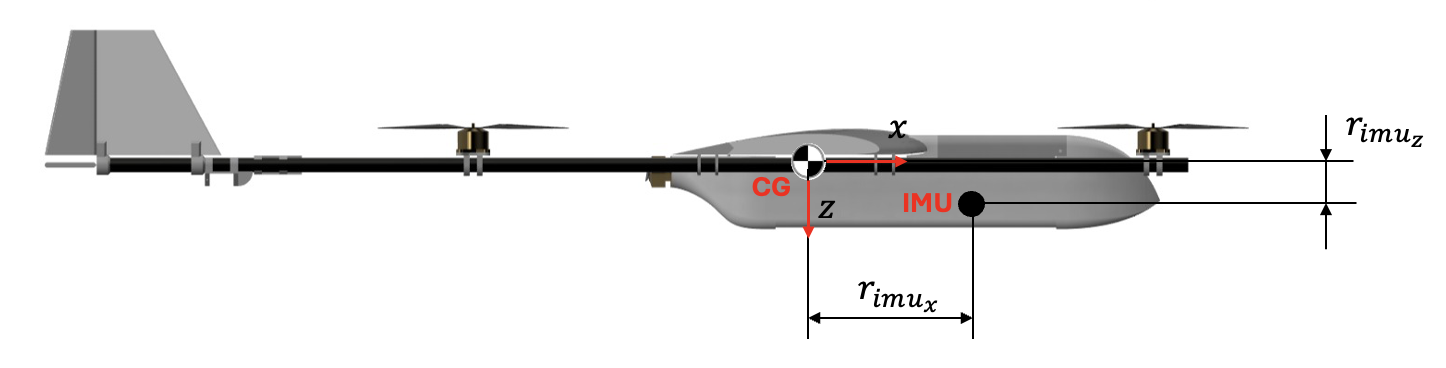
\includegraphics[width=\columnwidth]{displacement.png}
      \caption{Misalignment of the IMU relative to the CG.}
      \label{fig:imu_offset}
\end{figure}

The initial moments of inertia were estimated from the mass properties of a three-dimensional (CAD, \textit{Computer-Aided Design}) model of the aircraft, developed in the SolidWorks \textit{software}, and subsequently refined by the identification process.

\subsection{Dynamic Simulation of the Model}

The set of nonlinear differential equations that describes the dynamics of the quadrotor mode was implemented in MATLAB. The model was structured into blocks that compute the propulsion forces and moments from the bench curves, apply the aerodynamic drag, integrate the rotational and translational equations of motion (via 4th-order Runge-Kutta), and propagate the Euler kinematics, according to the diagram of Figure~\ref{fig:model_diagram}.

The simulation constitutes the central element of the estimation method: it generates the predicted response of the model ($y$) for a given control input. This response is compared with the actual response of the aircraft ($z$) to form the residual vector that the optimization algorithm minimizes.

\section{Results and Discussion}
\label{sec:resultados}

The application of the nonlinear least-squares method to the flight data in quadrotor mode allowed the estimation of the parameters of the dynamic model.

\subsection{Parameter Estimation Result}

The optimization process converged to the final parameter set $\Theta_{\text{OEM}}$, composed of the moments of inertia, the thrust and reaction-torque coefficients of each motor, and the rotational damping coefficients (Equation~\eqref{eq:theta}). The initial values ($\Theta_0$) and the estimated parameters are presented in Tables~\ref{tab:param_inercia},~\ref{tab:param_motor},~\ref{tab:param_motor_cm}, and~\ref{tab:param_rot}. The moments of inertia $J_{xx}$ and $J_{yy}$ increase by about 8.6\,\% and 16.6\,\% relative to the three-dimensional (CAD) model, respectively, reflecting the particularities of the hybrid VTOL configuration, in which the presence of the aerodynamic surfaces and the rear motor influences the mass distribution even when inactive in quadrotor mode.

\begin{table}[!htbp]
\caption{Moments and products of inertia.}
\label{tab:param_inercia}
\centering
\small
\begin{tabular}{lccccc}
\toprule
 & \multicolumn{2}{c}{\textbf{\boldmath$\Theta_0$}} & \multicolumn{2}{c}{\textbf{\boldmath$\Theta_{\text{OEM}}$}} & \\
\cmidrule(lr){2-3}\cmidrule(lr){4-5}
\textbf{Parameter} & \textbf{Value} & \textbf{CRB} & \textbf{Value} & \textbf{CRB} & \textbf{Unit} \\
\midrule
$J_{xx}$ & 0.0432 & 1.9\% & 0.0469 & 1.8\% & kg$\cdot$m$^2$ \\
$J_{yy}$ & 0.0844 & 1.7\% & 0.0984 & 1.7\% & kg$\cdot$m$^2$ \\
$J_{zz}$ & 0.1262 & 19.3\% & 0.1453 & 19.2\% & kg$\cdot$m$^2$ \\
$J_{xz}$ & 0.00157 & 70.3\% & 0.00261 & 30.4\% & kg$\cdot$m$^2$ \\
\bottomrule
\end{tabular}
\end{table}

\begin{table}[!htbp]
\caption{Thrust coefficients $c_{T_i}$ ($\times 10^{-7}$~N/RPM$^2$) per motor.}
\label{tab:param_motor}
\centering
\small
\begin{tabular}{lcccc}
\toprule
 & \multicolumn{2}{c}{\textbf{\boldmath$\Theta_0$}} & \multicolumn{2}{c}{\textbf{\boldmath$\Theta_{\text{OEM}}$}} \\
\cmidrule(lr){2-3}\cmidrule(lr){4-5}
\textbf{Parameter} & \textbf{Value} & \textbf{CRB} & \textbf{Value} & \textbf{CRB} \\
\midrule
$c_{T_1}$ & 1.76 & 1.2\% & 1.87 & 1.1\% \\
$c_{T_2}$ & 1.76 & 1.2\% & 1.86 & 1.1\% \\
$c_{T_3}$ & 1.76 & 1.3\% & 1.86 & 1.3\% \\
$c_{T_4}$ & 1.76 & 1.2\% & 1.89 & 1.2\% \\
\bottomrule
\end{tabular}
\end{table}

\begin{table}[!htbp]
\caption{Reaction-torque coefficients $c_{M_i}$ ($\times 10^{-9}$~N$\cdot$m/RPM$^2$) per motor.}
\label{tab:param_motor_cm}
\centering
\small
\begin{tabular}{lcccc}
\toprule
 & \multicolumn{2}{c}{\textbf{\boldmath$\Theta_0$}} & \multicolumn{2}{c}{\textbf{\boldmath$\Theta_{\text{OEM}}$}} \\
\cmidrule(lr){2-3}\cmidrule(lr){4-5}
\textbf{Parameter} & \textbf{Value} & \textbf{CRB} & \textbf{Value} & \textbf{CRB} \\
\midrule
$c_{M_1}$ & 5.04 & 47.4\% & 3.38 & 26.1\% \\
$c_{M_2}$ & 5.04 & 54.7\% & 3.16 & 25.5\% \\
$c_{M_3}$ & 5.04 & 42.9\% & 3.92 & 29.5\% \\
$c_{M_4}$ & 5.04 & 48.1\% & 3.47 & 27.3\% \\
\bottomrule
\end{tabular}
\end{table}

\begin{table}[!htbp]
\caption{Rotational damping coefficients.}
\label{tab:param_rot}
\centering
\small
\begin{tabular}{lccccc}
\toprule
 & \multicolumn{2}{c}{\textbf{\boldmath$\Theta_0$}} & \multicolumn{2}{c}{\textbf{\boldmath$\Theta_{\text{OEM}}$}} & \\
\cmidrule(lr){2-3}\cmidrule(lr){4-5}
\textbf{Parameter} & \textbf{Value} & \textbf{CRB} & \textbf{Value} & \textbf{CRB} & \textbf{Unit} \\
\midrule
$c_p$ & 0.5 & 32.9\% & 6.85 & 2.3\% & s$^{-1}$ \\
$c_q$ & 0.5 & 22.5\% & 4.68 & 2.2\% & s$^{-1}$ \\
$c_r$ & 0.5 & 7.7\% & 0.81 & 3.6\% & s$^{-1}$ \\
\bottomrule
\end{tabular}
\end{table}

The thrust coefficients $c_{T_i}$ increase to approximately $1.87\times10^{-7}$~N/RPM$^2$, correcting the underestimation of the EEM, while the reaction-torque coefficients $c_{M_i}$ decrease by about 30\,\% relative to the bench, reflecting the overestimation of the torque measured in a static test. Among the damping coefficients, $c_r$ (yaw) is the smallest, consistent with the low authority and lower observability of this axis; the reaction-torque coefficients $c_{M_i}$ and the product of inertia $J_{xz}$, associated with yaw, exhibit the largest relative deviations (above 20\,\%, by the Cramér--Rao bound), whereas $J_{xx}$, $J_{yy}$, $c_{T_i}$, and the damping coefficients remain below 5\,\%.

\subsection{Validation}
The validation of the identified model was carried out by comparing the simulated response with a set of flight data in quadrotor mode not used in the estimation process. Figures~\ref{fig:pqr_val} and~\ref{fig:acc_val} present, for the angular rates and the specific forces, the comparison between the measured data and the responses of the initial model with $\Theta_0$, the EEM, and the final OEM, highlighting the progressive improvement of the estimation.

\begin{figure}[!htbp]
    \centering
    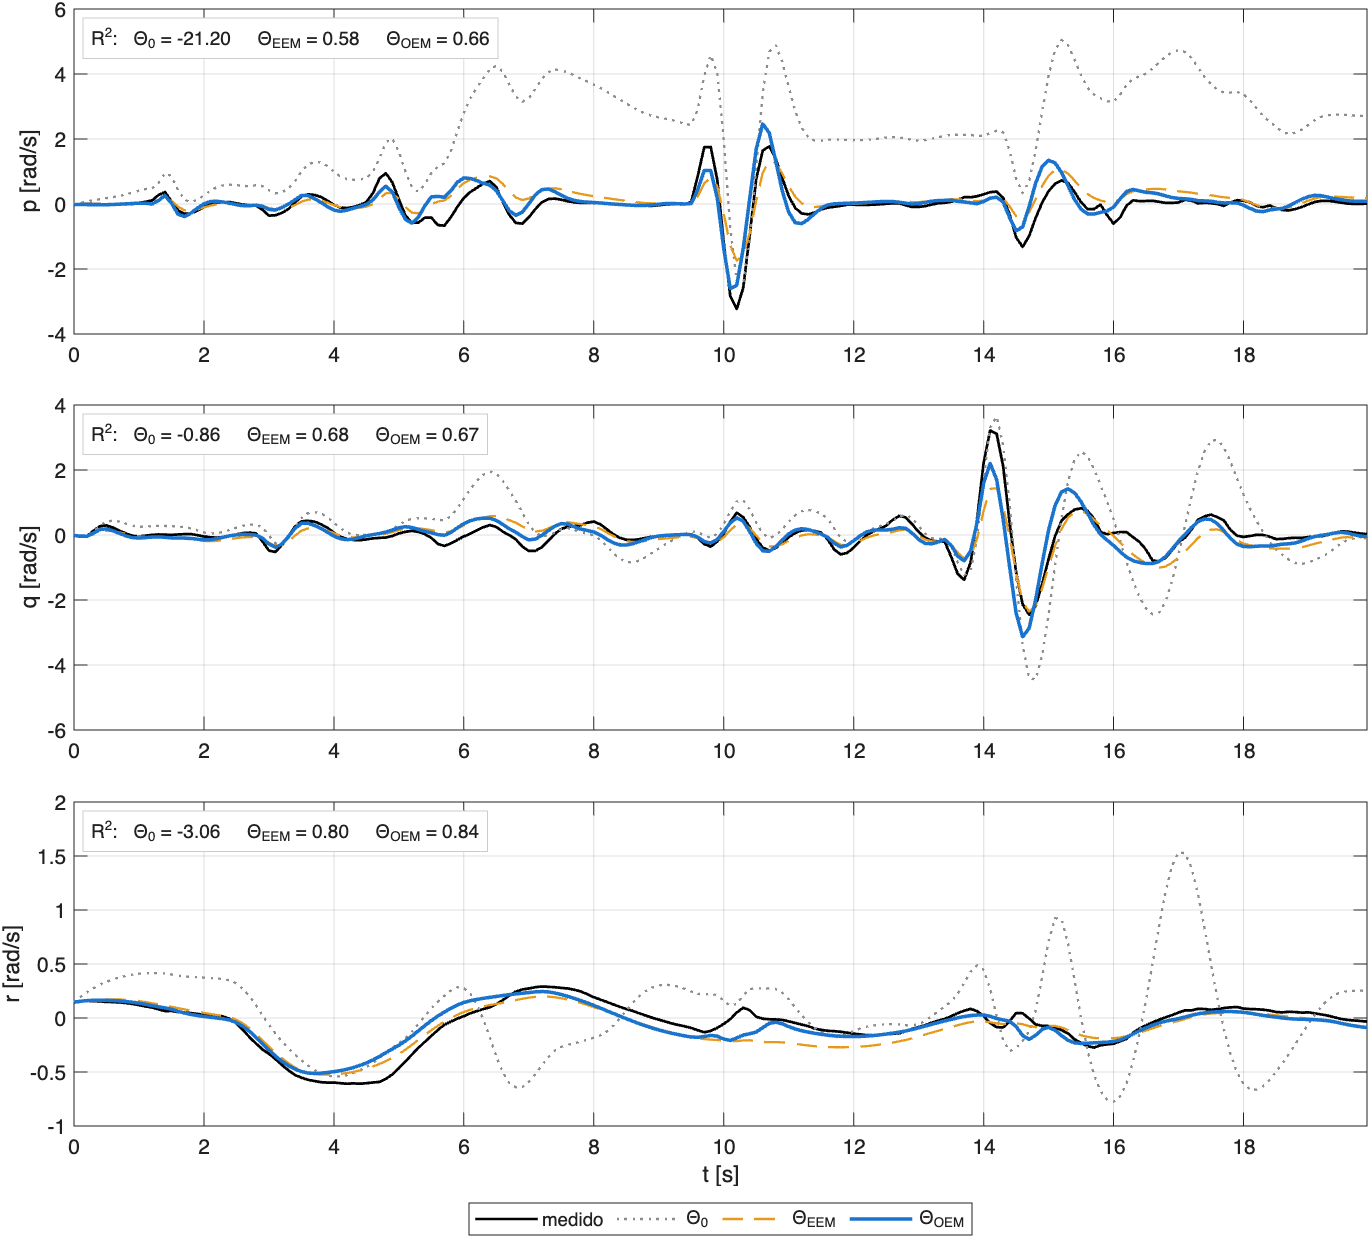
\includegraphics[width=\columnwidth]{id_comp_rates.png}
    \caption{Angular rates: comparison of the responses of the models {\mathversion{normal}$\Theta_0$}, {\mathversion{normal}$\Theta_{\text{EEM}}$}, and {\mathversion{normal}$\Theta_{\text{OEM}}$} against the measurements, on the validation segment.}
    \label{fig:pqr_val}
\end{figure}

\begin{figure}[!htbp]
    \centering
    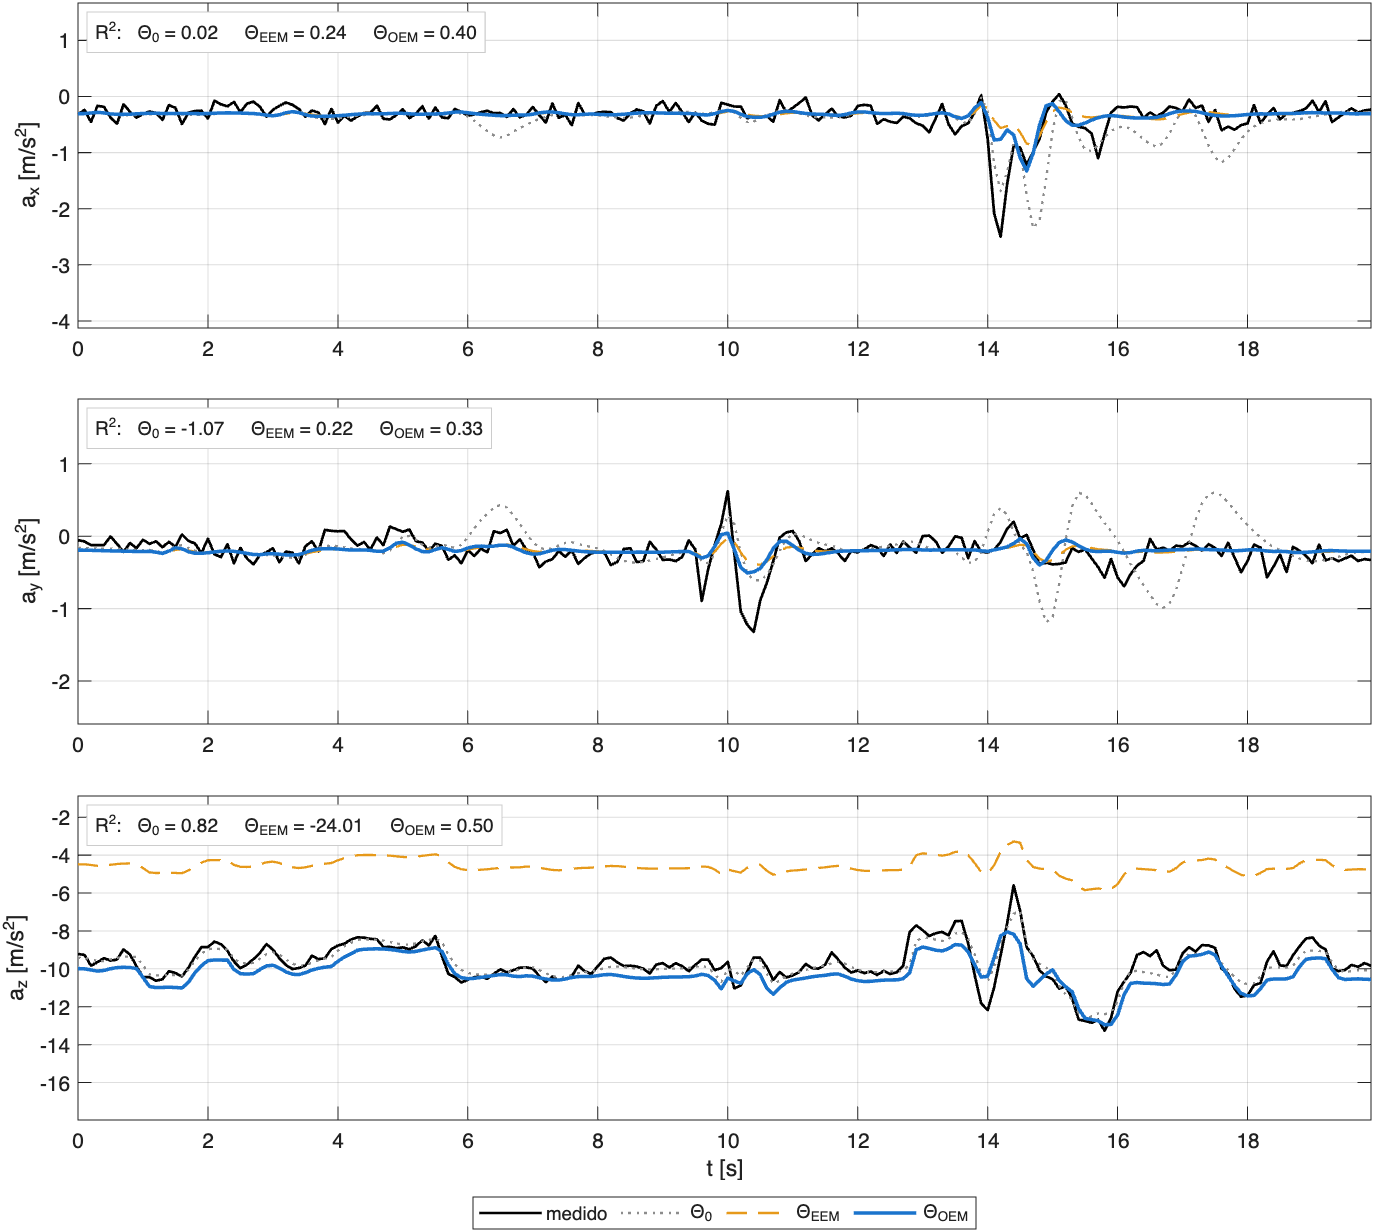
\includegraphics[width=\columnwidth]{id_comp_acc.png}
    \caption{Accelerations (IMU specific force): comparison of the responses of the models {\mathversion{normal}$\Theta_0$}, {\mathversion{normal}$\Theta_{\text{EEM}}$}, and {\mathversion{normal}$\Theta_{\text{OEM}}$} against the measurements, on the validation segment.}
    \label{fig:acc_val}
\end{figure}

The coefficient of determination $R^2$ obtained for each channel on the validation segment, for the initial model $\Theta_0$ and the final model $\Theta_{\text{OEM}}$, is presented in Table~\ref{tab:r2_val}. The initial model exhibits a strongly negative $R^2$ in the rates (reaching $-21.2$ in $p$), indicating that, without the estimated parameters, the simulation diverges from the measurements. In the final model, in turn, the angular rates show good agreement ($R^2$ between 0.66 and 0.84), with yaw ($r$) the best channel; the specific forces are reproduced moderately ($R^2$ between 0.33 and 0.50), reflecting the limits of the sensor model for the accelerations.

\begin{table}[!htbp]
\caption{Coefficient of determination $R^2$ per channel on the validation segment, for the initial model {\mathversion{normal}$\Theta_0$} and the final model {\mathversion{normal}$\Theta_{\text{OEM}}$}.}
\label{tab:r2_val}
\centering
\begin{tabular}{lcccccc}
\toprule
\textbf{Model} & $p$ & $q$ & $r$ & $a_x$ & $a_y$ & $a_z$ \\
\midrule
$\Theta_0$ (initial) & $-21.2$ & $-0.86$ & $-3.06$ & $0.02$ & $-1.07$ & $0.82$ \\
$\Theta_{\text{OEM}}$ (final) & $0.66$ & $0.67$ & $0.84$ & $0.40$ & $0.33$ & $0.50$ \\
\bottomrule
\end{tabular}
\end{table}

The results demonstrate good agreement between the identified model and the real data, indicating that the model adequately captures the dynamics of the quadrotor mode, including the coupling effects and the asymmetries arising from the hybrid VTOL configuration. This validation confirms that the model is suitable to serve as a basis for the design of controllers for the vertical takeoff and landing phases.

\section{Conclusion}
\label{sec:conclusao}

This work presented the identification of the dynamic model of the quadrotor mode of a hybrid-configuration VTOL UAV, taking into account the geometric and inertial particularities arising from the presence of aerodynamic surfaces and a cruise motor on the aircraft. Using the M4V methodology and the progressive multi-window output-error method, it was possible to estimate the parameters of a nonlinear model from real flight data.

From initial constants obtained by physical measurements and bench tests, the physical motor model and the allocation matrix reconstructed the control efforts directly from the PWM commands, while the moments of inertia $J_{xx}$ and $J_{yy}$, the thrust and reaction-torque coefficients of each motor, and the rotational damping coefficients were refined by the optimization. The validation with independent flight data showed coefficients of determination of 0.66, 0.67, and 0.84 in the roll, pitch, and yaw rates, confirming the predictive capability of the model. The Cramér--Rao analysis identifies yaw as the axis of lowest observability, with the reaction-torque coefficients among the least well-determined parameters, consistent with the low control authority of this axis in the H-frame configuration.

The identified model constitutes the basis for developing control algorithms and an autopilot (AP) for the autonomous vertical takeoff and landing phases. Future work includes the design of the attitude and altitude controllers, as well as the extension of the identification to the transition and fixed-wing modes.

\section*{Acknowledgments}
The authors thank the Instituto Tecnológico de Aeronáutica (ITA) for supporting the development of this work.

\begin{thebibliography}{99}

\bibitem{c1} V. Klein and E. A. Morelli, \textit{Aircraft System Identification: Theory and Practice}. Reston, VA, USA: AIAA, 2006, doi: 10.2514/4.861505.

\bibitem{c2} R. V. Jategaonkar, \textit{Flight Vehicle System Identification: A Time Domain Methodology}. Reston, VA, USA: AIAA, 2006, ISBN: 1-56347-836-6.

\bibitem{c3} M. B. Tischler and R. K. Remple, \textit{Aircraft and Rotorcraft System Identification}, 2nd ed. Reston, VA, USA: AIAA, 2012, doi: 10.2514/4.868207.

\bibitem{c4} N. V. Hoffer, C. Coopmans, A. M. Jensen, and Y. Chen, ``A survey and categorization of small low-cost unmanned aerial vehicle system identification,'' \textit{J. Intell. Robot. Syst.}, vol. 74, no. 1--2, pp. 129--145, 2014, doi: 10.1007/s10846-013-9931-6.

\bibitem{c5} O. Arifianto and M. Farhood, ``Development and modeling of a low-cost unmanned aerial vehicle research platform,'' \textit{J. Intell. Robot. Syst.}, vol. 80, no. 1, pp. 139--164, Oct. 2015, doi: 10.1007/s10846-014-0145-3.

\bibitem{c7} D. J. Grymin and M. Farhood, ``Two-step system identification and trajectory tracking control of a small fixed-wing UAV,'' \textit{J. Intell. Robot. Syst.}, vol. 83, no. 1, pp. 105--131, 2016, doi: 10.1007/s10846-015-0298-8.

\bibitem{c8} S. Bouabdallah and R. Siegwart, ``Full control of a quadrotor,'' in \textit{Proc. IEEE/RSJ Int. Conf. Intell. Robots Syst. (IROS)}, Oct. 2007, pp. 153--158, doi: 10.1109/IROS.2007.4399042.

\bibitem{c9} D. Mellinger and V. Kumar, ``Minimum snap trajectory generation and control for quadrotors,'' in \textit{Proc. IEEE Int. Conf. Robot. Autom. (ICRA)}, May 2011, pp. 2520--2525, doi: 10.1109/ICRA.2011.5980409.

\bibitem{c11} B. P. Graesdal, ``Full nonlinear system identification for a vertical-takeoff-and-landing unmanned aerial vehicle,'' M.S. thesis, Dept. Eng. Cybern., Norwegian Univ. Sci. Technol. (NTNU), Trondheim, Norway, 2022.

\bibitem{c12} L. E. Hale, M. Patil, and C. J. Roy, ``Aerodynamic parameter identification and uncertainty quantification for small unmanned aircraft,'' \textit{J. Guid. Control Dyn.}, vol. 40, no. 3, pp. 680--691, 2017, doi: 10.2514/1.G000582.

\bibitem{cBeard} R. W. Beard and T. W. McLain, \textit{Small Unmanned Aircraft: Theory and Practice}. Princeton, NJ, USA: Princeton Univ. Press, 2012, ISBN: 978-0-691-14921-9.

\bibitem{c13} Q. Quan, \textit{Introduction to Multicopter Design and Control}. Singapore: Springer, 2017, doi: 10.1007/978-981-10-3382-7.

\end{thebibliography}

\EOD

\end{document}
